\documentclass[11pt]{jarticle}
\usepackage[dvipdfmx]{graphicx}        % 画像を扱えるようにする.
\graphicspath{{./img/}}
\usepackage{ascmac}                    % 丸枠を使用可能にする.
\usepackage{color}                     % 色文字を有効にする.
\usepackage{url}                       % \url{}を使用可能にする.
\usepackage{fancyvrb}                  % \Verbatimを使用可能にする.
\usepackage{fancybox}                  % itembox等を使用可能にする.
\usepackage{type1cm}
\usepackage{listings,jlisting}
\lstset{
  language=C,
  basicstyle=\ttfamily\scriptsize,
  commentstyle={\itshape \color[cmyk]{1,0.4,1,0}},
  classoffset=1,
  keywordstyle={\bfseries \color[cmyk]{0,1,0,0}},
  stringstyle={\ttfamily \color[rgb]{0,0,1}},
  frame=tRBl,
  framesep=5pt,
  showstringspaces=false,
  numbers=left,
  stepnumber=1,
  numberstyle=\tiny,
  tabsize=2,
  breaklines = true,
  escapeinside={(*@}{@*)},
}
\usepackage[junior]{gaiyo}             % styファイルは既存のものを使用.
%
% ここからマニュアル用スタイル設定.
\makeatletter
\gdef\@id{}
\gdef\@author{}
%
\def\hdtype#1{\gdef\hd@type{#1}}
\def\@maketitle{\begin{center}
  \vspace{\baselineskip}
  {\fontsize{16pt}{0.6565cm}\selectfont \bfseries
    \@title \par
  }
\end{center}
}
\makeatother
% ここまでマニュアル用スタイル設定.
%
% タイトルとヘッダの設定.
\title{ネットワーク講習}
\hdtype{ネットワーク講習}
%
% ここから文書開始.
%
\begin{document}
\maketitle
%
% ここから本文.
% 

\section{はじめに}

\subsection{ネットワークとは}

	「ネットワーク」とは,なにかとなにかが網の目のようになにかによって繋がっている状態のことであり,なにかを運ぶためのものである.
	単にネットワークというと,物流・道路・神経などいろいろなものがあるが,特に「コンピュータネットワーク」においては,コンピュータとコンピュータが網の目のようにケーブルなどの通信媒体によって繋がっており,データを運ぶためのものであると定義できる.

\subsection{ネットワークの利点}

	コンピュータネットワークを用いると,メールやファイルのやり取りが行えるだけではなく,他のコンピュータに繋がっているプリンタを使用したり,他のコンピュータにデータを処理させることもできる.

	メールやファイル,印刷したいデータなど,コンピュータやユーザが持つものを「リソース」と呼ぶ.
コンピュータネットワークを利用する最大の利点は,こうしたリソースを複数のコンピュータで共有することであるといえる.


\subsection{プロトコル}
	人と人とが会話をするとき,お互いが異なる言語を用いてしまうと正しく意思疎通を行うことができない.つまり,人間同士の会話が成立するためには「お互いが理解できる言語を用いる」という暗黙的なルールが存在していなければならない.
	
	同様に,コンピュータの世界においても,複数のコンピュータ同士がネットワークを介して通信を行うときには共通のルールが必要となる.柔軟な対応ができる人間とは異なり,コンピュータは機械であるため,通信を行うためには事前にありとあらゆるルールを決めておく必要がある.
	
	例えば,メールを送信するときのルールやファイルのやり取りを行うときのルール,通信相手を特定するときのルール,通信経路を選択するときのルール,通信途中でデータが壊れてしまったときのルール,更には,通信を行う際に用いるケーブルの種類や電気信号の変換方法など,様々な取り決めやルールが存在している.これらのルールのことを「プロトコル」と呼び,使用するプロトコルが異なれば正しく通信を行うことができない.
\section{OSI参照モデル}

\subsection{OSI参照モデル}
	ネットワーク機器や端末を開発するメーカーがそれぞれ好き勝手なプロトコルを用いてしまうと,メーカーの異なる機器同士で通信が行えなくなってしまうという問題が起こる.そこで,世界的にプロトコルの標準化が進められ,「OSI参照モデル」というプロトコルの設計モデルが1984年に国際標準化機構(ISO)によって制定された.
	
	現在では,プロトコルの設計モデルとして「TCP/IPモデル」が一般的に普及している.TCP/IPモデルは必ずしもOSI参照モデルに準拠している訳ではないが,データ通信における流れとしてはOSI参照モデルと類似している部分が多い.そのため,OSI参照モデルはネットワーク通信を行う際の基本的な考え方であるとして今でも広く浸透している.今回の講習でも,分かりやすさのためにOSI参照モデルを用いて説明を行う.


\subsection{階層構造}
	一度のデータ通信を行うとき,必要となるプロトコルは一つだけではなく,複数のプロトコルが使用されている.
	OSI参照モデルでは,それぞれのプロトコルの役割に応じてデータ通信を七つの段階に分類している.各段階のことを「レイヤ」と呼び,ネットワークによるデータ通信は各レイヤごとの複数のプロトコルで実現される.OSI参照モデルにおける各レイヤの名称と役割を表\ref{tab:osi}に示す.

	\begin{table}[htb]
		\begin{center}
			\caption{OSI階層モデルの各レイヤと役割}
			\begin{tabular}{|c|c|c|} \hline
				レイヤ & 名称 & 役割 \\ \hline
				レイヤ7 & アプリケーション層 & アプリケーションソフト間での通信を規定 \\ 
				レイヤ6 & プレゼンテーション層 & データ形式に関する規定 \\
				レイヤ5 & セッション層 & 通信の開始/終了に関する規定 \\
				レイヤ4 & トランスポート層 & 通信の品質を確保するための通信手順を規定 \\
				レイヤ3 & ネットワーク層 & 異なるネットワーク間の通信を規定 \\
				レイヤ2 & データリンク層 & 同じネットワーク内の通信を規定 \\
				レイヤ1 & 物理層 & 接続のための物理的な規定 \\ \hline
			\end{tabular}
			\label{tab:osi}
		\end{center}
	\end{table}

	各レイヤは独立しており,レイヤのプロトコルの変更は他のレイヤに影響を及ぼさない.また,基本的には下位のレイヤは上位のレイヤを考慮して設計されており,上位のレイヤは下位のレイヤを意識する必要は無い.


\subsection{カプセル化}

	誰かに宅配便を送る場合,送る側がまず贈り物を梱包材に包み,ダンボールに入れて,宛先や送り主を書いた配達表を貼ることで,配達員に宛先まで運んでもらう.宅配便を受け取った側は,配達表を剥がし,ダンボールから取り出して,梱包を解くという,送る側と逆の手順を踏むことで贈り物を正しく受け取ることができる.
	
	同様に,コンピュータがデータ通信を行う場合も,送りたいデータに対して制御情報(ヘッダ)を付け加える作業が必要となる.制御情報とは,送信先・送信元のアドレスや,それぞれのプロトコルで必要となる情報などである.
	
	OSI参照モデルでは,送信側が各レイヤにおいて7から1の順番でそれぞれの手順をこなし,送りたいデータに制御情報を付け加えていく.このように,各レイヤにおいてデータに制御情報を付け加えていく作業を「カプセル化」と呼ぶ.受信側は,各レイヤにおいて1から7の順番でそれぞれの手順をこなし,送信側とは逆の順序で制御情報を取り除いていくことで,最終的に目的のデータを受け取ることができる.
	OSI参照モデルにおけるカプセル化を用いたデータ通信の流れを図\ref{fig:capsule}に示す.

	\begin{figure}[htb]
		\begin{center}
			\includegraphics[width=160mm]{osi_capsule.eps}
		\end{center}
		\caption{OSI参照モデルによるカプセル化の流れ}
		 \label{fig:capsule}
	\end{figure}


\subsection{TCP/IPモデル}
		
	現在インターネットで広く用いられているプロトコル群はIETFが制定したTCP/IPプロトコル群であり,これらは「TCP/IPモデル」がベースとなっている.OSI参照モデルが七つのレイヤで構成されていたのに対し,TCP/IPモデルは四つのレイヤで構成される.OSI参照モデルとTCP/IPモデルの階層の対応を図\ref{fig:tcp_layer}に,また,TCP/IPで用いられるプロトコルの例を表\ref{tab:tcp}に示す.
	
	\begin{figure}[htb]
		\begin{center}
			\includegraphics[width=160mm]{tcp_layer.eps}
		\end{center}
		\caption{OSI参照モデルの7階層とTCP/IPモデルの4階層}
		 \label{fig:tcp_layer}
	\end{figure}

	\begin{table}[htb]
		\begin{center}
			\caption{TCP/IPモデルのプロトコル例}
			\begin{tabular}{|c|c|c|} \hline
				レイヤ & 名称 & プロトコルの例 \\ \hline
				レイヤ4 & アプリケーション層 & HTTP,FTP,SMTP \\
				レイヤ3 & トランスポート層 & TCP,UDP \\
				レイヤ2 & インターネット層 & IP,ARP \\
				レイヤ1 & インターフェース層 & Ethernet,PPP \\ \hline
			\end{tabular}
			\label{tab:tcp}
		\end{center}
	\end{table}
	
	TCP/IPモデルのレイヤ4は,OSI参照モデルでいうところのレイヤ5,6,7の部分に対応し,また,TCP/IPモデルのレイヤ1は,OSI参照モデルでいうところのレイヤ1,2の部分に対応している.注意してほしいのは,実際にはTCP/IPモデルとOSI参照モデルはまったく別のプロトコル設計モデルだということである.例えば.TCP/IPモデルのインターネット層とOSI参照モデルのネットワーク層は,役割は似ているが同一のものではない.
	
	以降では,基本的にTCP/IPプロトコル群を利用したネットワークについて説明する.
	
	
	
\section{Internet Protocol}
IP(Internet Protocol)はTCP/IPモデルにおいてデータの送受信を担うプロトコルである.OSI参照モデルにおけるレイヤ3(ネットワーク層)に相当する役割を持ち,IPアドレスと呼ばれるIP独自の論理アドレスに基づいてデータをやり取りすることを特徴としている.IPは異なるネットワークに属する通信相手までデータを届ける機能を持ち,物理的に遠く離れた相手との通信経路を確立する.TCP/IPモデルの中核となる重要なプロトコルである.

\subsection{IPアドレスとは}
IPアドレスはIPでの通信に利用されるアドレスである.機器を示す情報(誰)だけでなく,属するネットワークの情報(何処)も含んでいるという特徴があり,異なるネットワークへデータを転送するときに経路の探索が容易にできるような仕組みになっている.郵便配達における住所のようなものであるといえる.

レイヤ2(データリンク層)のEthernetでは,機器ごとに割り振られたMACアドレス(物理アドレス)を利用して通信を行っていたが,MACアドレスは機器を示す情報(誰)しか含んでおらず,MACアドレスからその機器が属するネットワーク(何処)を知ることはできなかった.IPであれば異なるネットワークに存在する機器であっても,その機器が属するネットワークを割り出し通信経路を探し出すことができる.

IPアドレスにはIPv4アドレスとIPv6アドレスという二つの形式があるが,以下の項では現在の主流であるIPv4アドレスについて説明する.

\subsection{IPアドレスの構造}
IPアドレスは32桁の2進数(32ビット)の番号として表される.しかし,そのままでは人間が読み取ることは困難であるため,通常はビット列を1バイト(8ビット)ごとに区切り,10進数を用いて表記する(表\ref{tab:ip_des}).1バイトの区切りのことをオクテットと呼び,32ビットのIPアドレスは4オクテット構成となる.

\begin{table}[htb]
  \begin{center}
    \caption{IPアドレスの表記}
    \begin{tabular}{|l||c|} \hline
      2進数 & 10011110.11011001.01001101.11100001 \\ \hline
      10進数 & 158.217.77.225 \\ \hline
    \end{tabular}
    \label{tab:ip_des}
  \end{center}
\end{table}

\begin{figure}[htb]
  \begin{center}
    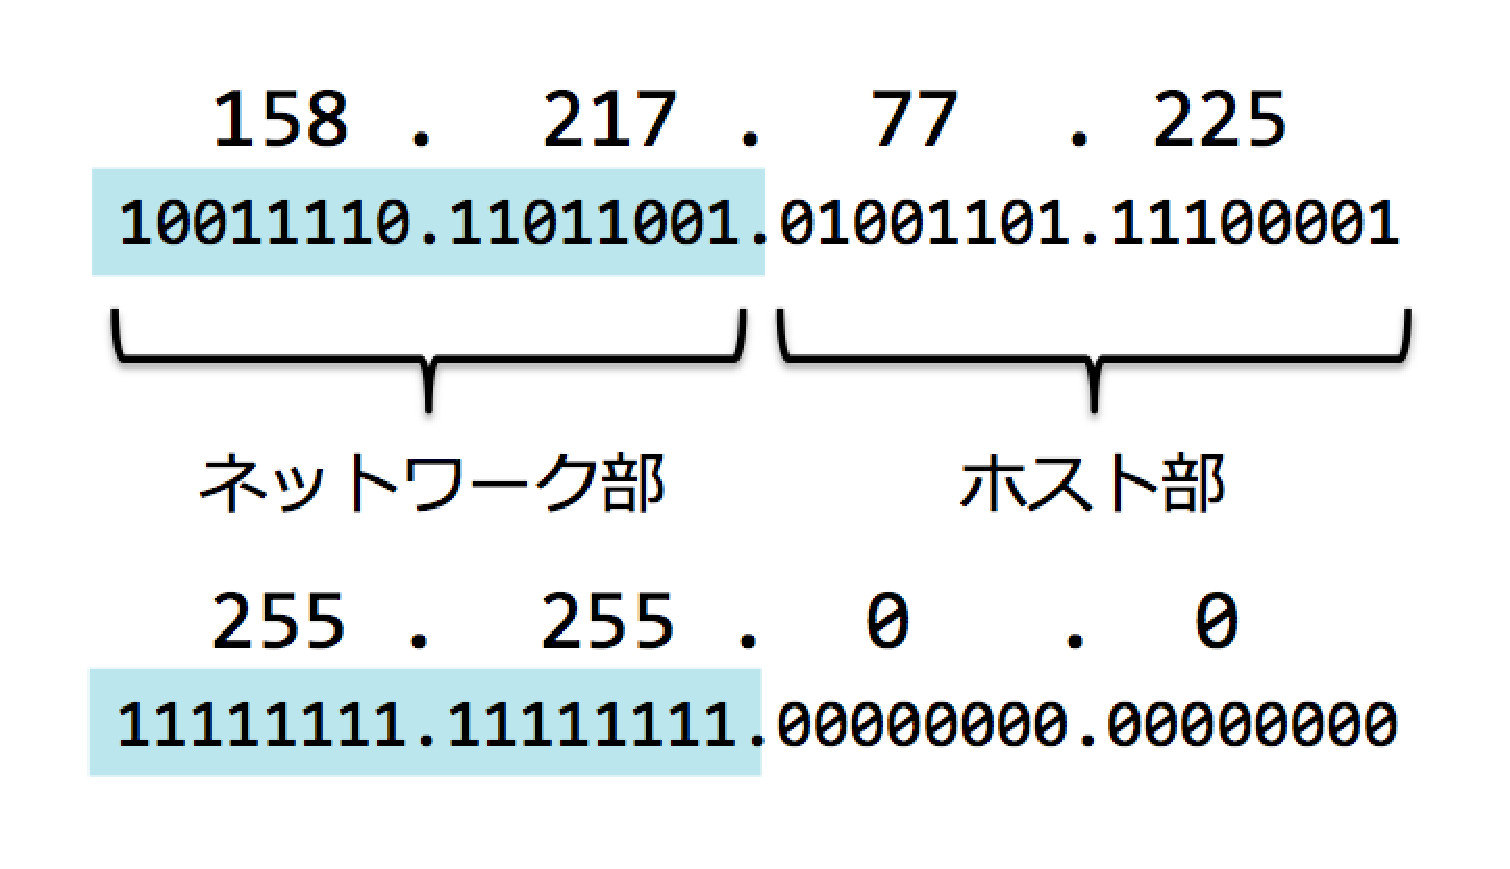
\includegraphics[width=82mm, bb=0 0 709 401]{netmask1.eps} 
  \end{center}
  \caption{ネットワーク部とホスト部}
  \label{fig:netmask1}
\end{figure}

IPアドレスはホストが属するネットワークを示す『ネットワークアドレス』と,機器を特定する『ホストアドレス』から構成される階層型アドレスである.図\ref{fig:netmask1}の例では,「158.217.77.225は,158.217.0.0ネットワークにある77.225番の機器である.」と解釈することができる.何処(158.217.0.0ネットワーク)の誰(77.225番)という情報があれば,相手が自分と同じネットワークにいるのか,あるいは遠く離れたネットワークに居るのか,などを見分けることができるため,通信経路の探索が容易になる.

ネットワークアドレスは全ネットワーク内でユニークなものである必要があり,インターネットの場合ではNIC(Network Information Center)等の組織が企業やプロバイダに対してネットワークアドレスを割り振っている.一方,ホストアドレスは各ネットワークの管理者が任意の機器に割り振ることができ,そのネットワーク内でユニークなものでさえあれば良い.

\subsection{クラスフルアドレッシング}

先程の例(158.217.77.225)では,IPアドレスの左から16ビットをネットワークアドレスを示す『ネットワーク部』,残りのビットをホストアドレスを示す『ホスト部』としていたが,この境目はIPアドレスが属するアドレスクラス(表\ref{tab:ip_class})によって決定される.

\begin{table}[htb]
  \begin{center}
    \caption{アドレスクラス}
    \begin{tabular}{|c|c|c|c|c|c|} \hline
      クラス & アドレス範囲 & ネットワーク部 & ホスト数  & 用途 \\ \hline \hline
      A & 0.0.0.0 〜 127.255.255.255 & 8ビット & 16,777,214 & 大規模ネットワーク用  \\ \hline 
      B & 128.0.0.0 〜 191.255.255.255 & 16ビット & 65,534 & 中規模ネットワーク用  \\ \hline 
      C & 192.0.0.0 〜 223.255.255.255 & 24ビット & 254 & 小規模ネットワーク用 \\ \hline 
      D & 224.0.0.0 〜 239.255.255.255 & - & - & マルチキャスト用 \\ \hline 
      E & 240.0.0.0 〜 255.255.255.255 & -  & - & 実験用 \\ \hline 
    \end{tabular}
    \label{tab:ip_class}
  \end{center}
\end{table}

ネットワーク部とホスト部の境目を示すビット列(例. 255.255.0.0)のことを『ネットマスク』と呼び,アドレスクラスを元にネットマスクを決定する方式を『クラスフルアドレッシング』と呼ぶ.

IPアドレスは32ビット固定であるため,ネットワーク部が大きくなればホスト部は小さくなり,そのネットワークに割り振れるホストの数は少なくなる.逆に,ネットワーク部が小さくなればホスト部は大きくなり,そのネットワークに割り振れるホストの数は多くなる.しかし,クラスAの場合では割り振れるホストの数が16,777,214台にもなり,一つのネットワークとして管理するにはあまりにも巨大になってしまうという問題がある.対応策として,次の項で説明する『サブネット』などの手法が用意されている.

\subsection{サブネット}
クラスフルアドレッシングのようなIPアドレスの分類はネットワークの規模に応じてIPアドレスを使い分けるために決められたものである.しかし,IPアドレスの値による固定的なネットマスクの分割ではあまり柔軟にネットワークを構築することはできず,クラスAやクラスBのネットワークの場合にはネットワークがあまりにも巨大になってしまう.

そこで,各ネットワークの管理者が自由にネットワークアドレスとホストアドレスを決定できるようにするために『サブネット分割』という手段が用いられる.既存のネットワークをさらに小さなネットワークに区切り,それを『サブネット』として扱うという手法である.いままではIPアドレスを『ネットワーク部』と『ホスト部』の2つに分けていたが,サブネットに区切った場合,IPアドレスは『ネットワーク部』,『サブネット部』,『ホスト部』の3つに分割されることになる(図\ref{fig:netmask2}).このとき,サブネット部の境目を示すビット列(例. 255.255.255.0)のことを『サブネットマスク』と呼ぶ.

\begin{figure}[htb]
  \begin{center}
    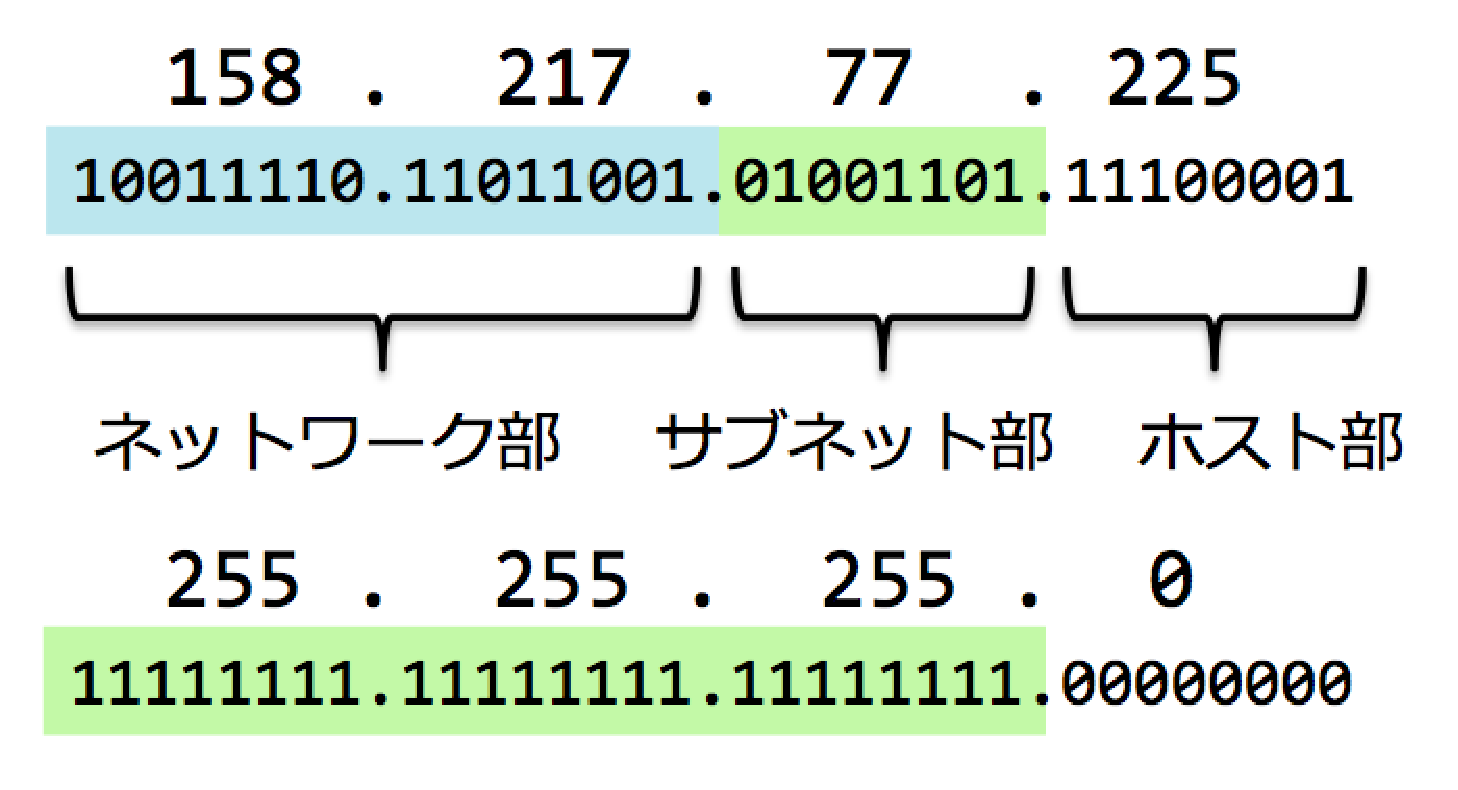
\includegraphics[width=82mm, bb=0 0 684 363]{netmask2.eps} 
  \end{center}
  \caption{サブネット分割}
  \label{fig:netmask2}
\end{figure}

アドレスクラスによって定められたネットマスクではなく,ネットワーク管理者が決めた自由なネットマスク(サブネットマスク)を使うことにより,ネットワークの規模などに応じて柔軟にネットワークを構築できるようになる.しかし,サブネットを使ったネットワークではネットマスクが環境ごとに異なるため,サブネットマスクをIPアドレスと同時に表記する必要がある.

\begin{itembox}[c]{サブネットマスクの表記法}
サブネットマスクの表記法にはいくつかの種類がある.
\begin{itemize}
    \item 192.168.1.52/11111111.11111111.11111111.00000000
    \item 192.168.1.52/255.255.255.0
    \item 192.168.1.52/0xffffff00
    \item 192.168.1.52/24
\end{itemize}
これら4種類の表記法はどれも同じサブネットマスクを表している.ソフトウェアによって様々な表記が使われるので,どれが出てきても意味が分かるようにしよう.
\end{itembox}

\subsection{予約済みアドレス}
IPアドレスの中にはどのホストにも割り振ることができない特別なアドレスが存在し,これらのアドレスのことを『予約済みアドレス』と呼ぶ.以下に各ネットワークごとに存在する2種類の予約済みアドレスについて説明する.

\begin{screen}
\begin{description}
 \item[ネットワークアドレス]\mbox{}\\ 
	    ホストアドレスのビットが全て0になるアドレス.これはネットワークそのものを表すアドレスであり,特定の機器ではなくネットワークそのものを指定したい場合に利用する.\\
 \fbox{例: 158.217.0.0(10011110.11011001.00000000.00000000)}
 \item[ブロードキャストアドレス]\mbox{}\\
	    ホストアドレスのビットが全て1になるアドレス.ネットワーク内の全てのホストを表すアドレスとなる. ネットワーク内の全ての機器に対してデータを送信したい場合に利用する.\\
\fbox{例: 158.217.255.255(10011110.11011001.11111111.11111111)}	    
\end{description}
\end{screen}

各ネットワークは必ずこれら2つの予約済みアドレスを持つため,ホスト部が\(n\)ビットだとするとホストに割り振れるアドレスは\(2^n-2\)個となる.予約済みアドレスはこれが全てではなく,他にもループバックアドレス(127.0.0.1)やプライベートアドレスといった特別なアドレスが予約されている.

\subsection{ifconfig/ipconfig}
ifconfig/ipconfigはIPネットワーク設定を確認したり,再設定したりするときに使うコマンドである.ネットワーク関係のコマンドとして最も頻繁に使われるものの一つで,ネットワーク管理には欠かせないコマンドである.情報の見方を是非頭に入れておこう.

Macではifconfigをターミナルから,Windowsではipconfigをコマンドプロンプトから実行する.

\begin{screen}
\begin{description}
 \item[Mac(ifconfig)]\mbox{}\\ 
  \begin{center}
    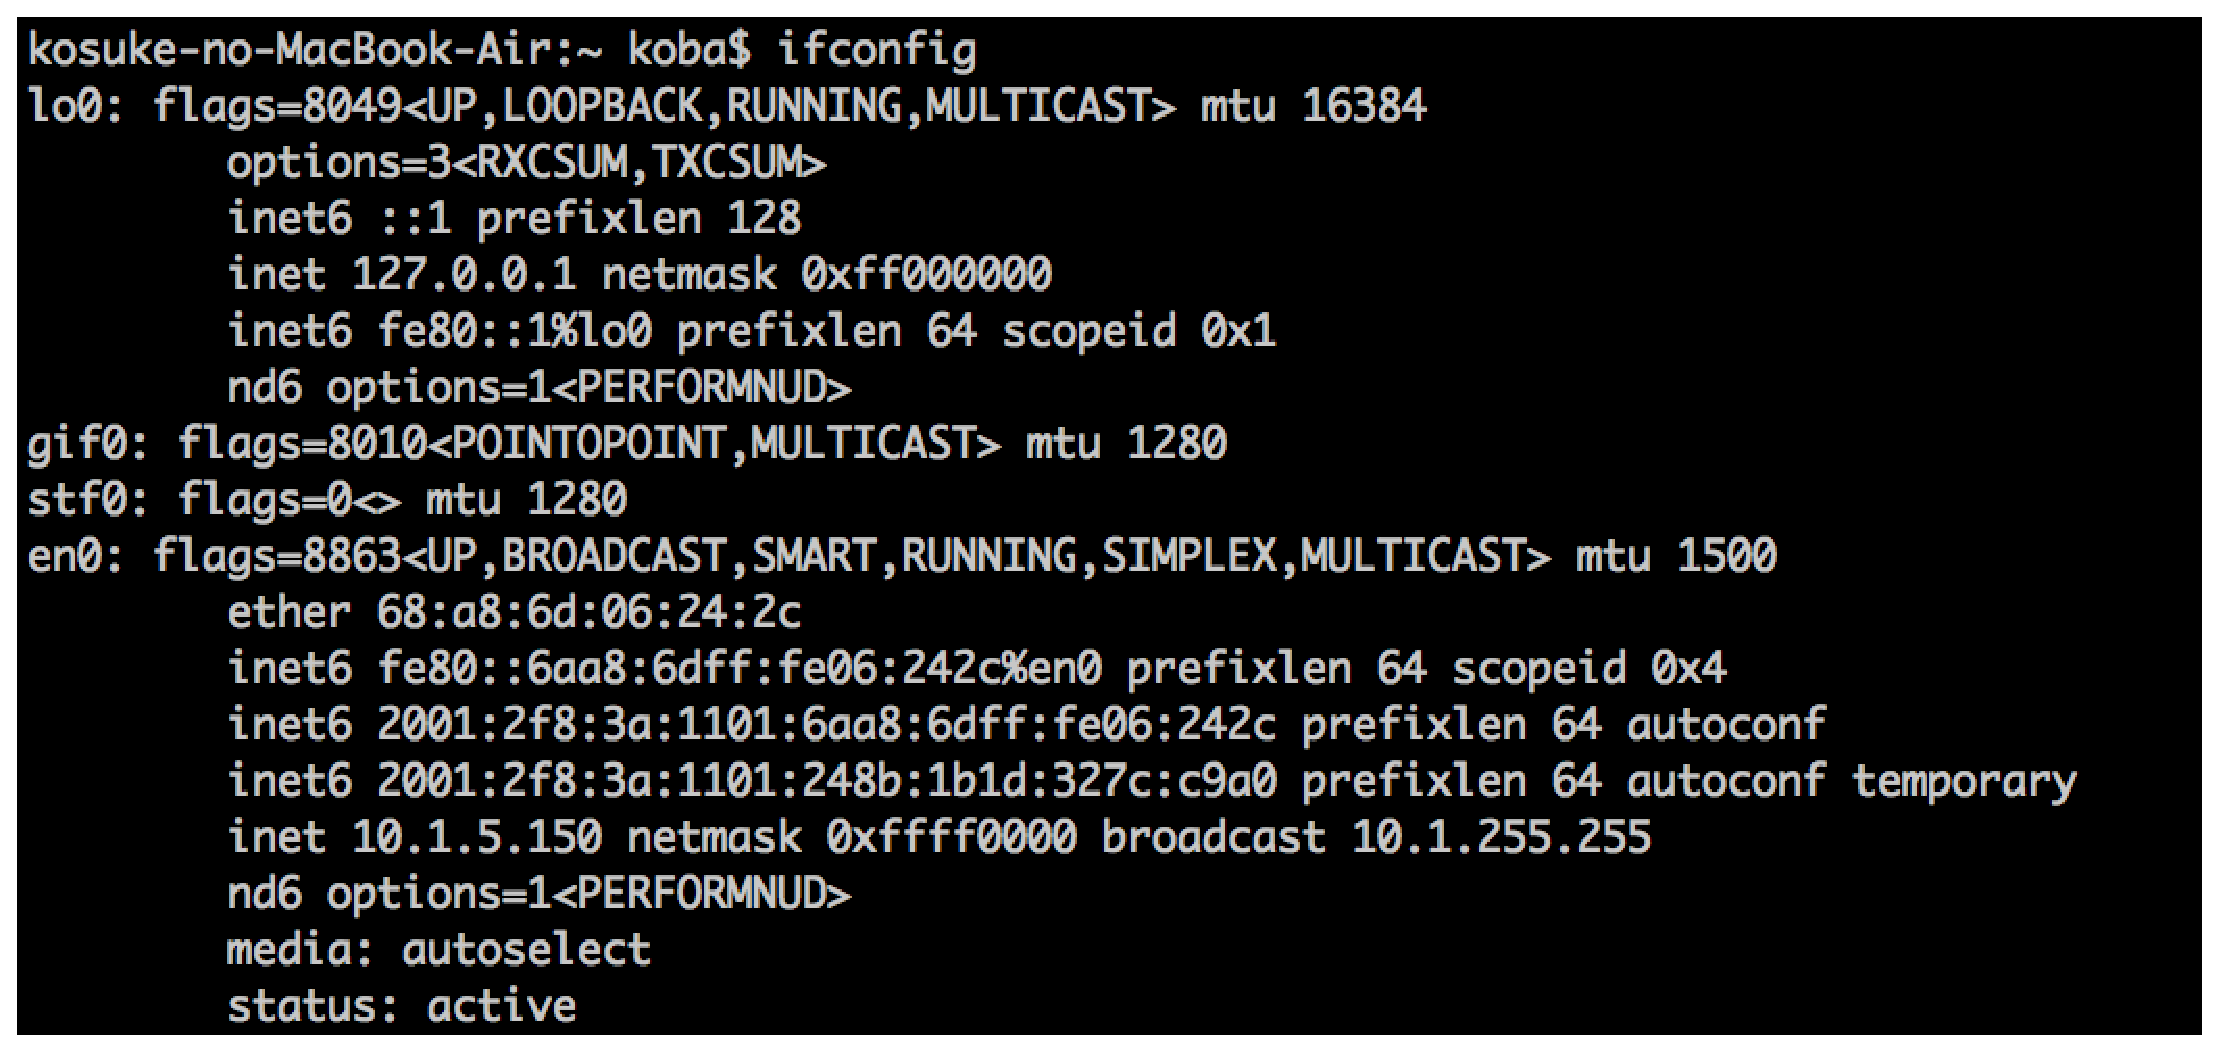
\includegraphics[width=140mm, bb=0 40 1049 469]{ifconfig.eps} 
  \end{center}
  上の実行例ではen0がネットワークに繋がる機器(NIC)となっている.etherの項にはMACアドレス,inet6の項にはIPv6についての情報が記載されている.\\
  IPアドレス(IPv4)についての情報はinetから始まる行に記載されている.\fbox{inet 10.1.5.150}は機器に割り振られたIPアドレスを表し,\fbox{netmask 0xffff0000}はサブネットマスクを表している.\\
 \item[Windows(ipconfig)]\mbox{}\\
     \begin{center}
    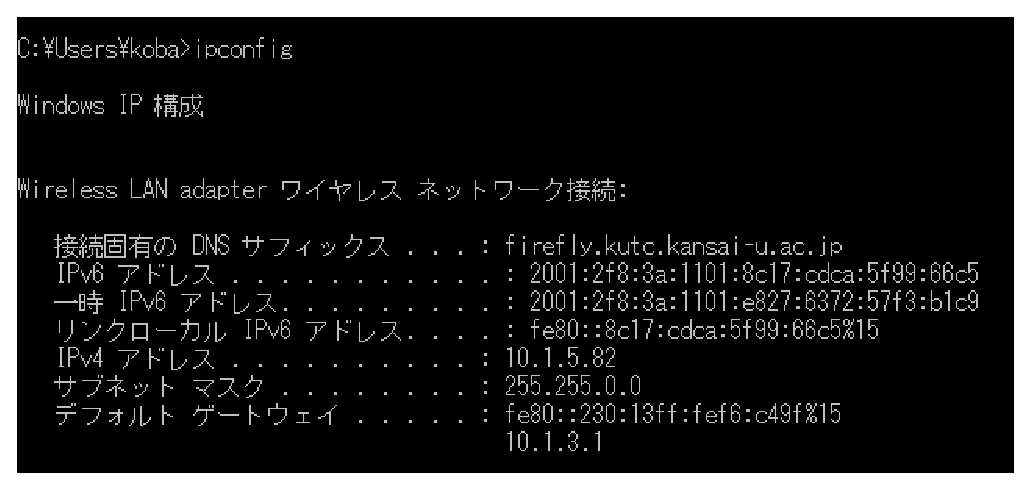
\includegraphics[width=138mm, bb=0 0 478 212]{ipconfig.eps} 
  \end{center}
  IPアドレス(IPv4)についての情報はIPv4アドレスから下の項に記載されている.\fbox{IPv4アドレス…: 10.1.5.82}は機器に割り振られたIPアドレスを表し,\fbox{サブネットマスク…: 255.255.0.0}は見ての通りサブネットマスクを表している.
\end{description}
\end{screen}

\subsection{DNS}
DNS(Domain Name Service)はIPアドレスとドメイン名の対応付けを行うサービスである.ドメイン名からIPアドレスを問い合わせること(正引き)と,IPアドレスからドメイン名を問い合わせること(逆引き)の両方を行うことができる.インターネットを利用する上でなくてはならない存在であり,現在のインターネットにとって必要不可欠なシステムの一つである.

ブラウザでWebページを閲覧するとき,ブラウザはIPアドレスを使ってWebサーバと情報のやり取りを行っている.しかし,ブラウザを利用しているユーザが直接IPアドレスを入力することは少ない.ユーザが入力するのは多くの場合,IPアドレスと比べて記憶し易いURI(例. https://www.firefly.kutc.kansai-u.ac.jp/xoops/)である.

URIからプロトコル名(https://)とディレクトリ名・ファイル名(/xoops/)を取り払ったものをドメイン名,厳密にはFQDN(完全修飾ドメイン名)と呼ぶ.ブラウザはこのドメイン名を使って目的のWebページのIPアドレスをDNSサーバに対して問い合わせ,IP通信を行っている.

ネットワークの設定の際にはDNSサーバ(及びセカンダリDNSサーバ)のIPアドレスが求められる.小林ゼミではDNSサーバ(10.1.3.21,10.1.3.80)を運用しており,ゼミ内ネットワークを使用する際にはこれらのDNSサーバのIPアドレスを設定する必要がある.

\subsection{FQDN}
FQDNとドメイン名は混同されがちであるが,厳密には異なるものである.ドメイン名はサーバが存在するネットワークを特定するための文字列であるが,FQDNはさらにホスト名をドメイン名に加えたものである.そのため,FQDNはホスト名とドメイン名に分割して考えることができる(図\ref{fig:URI_hostdomain}).

\begin{figure}[htb]
  \begin{center}
    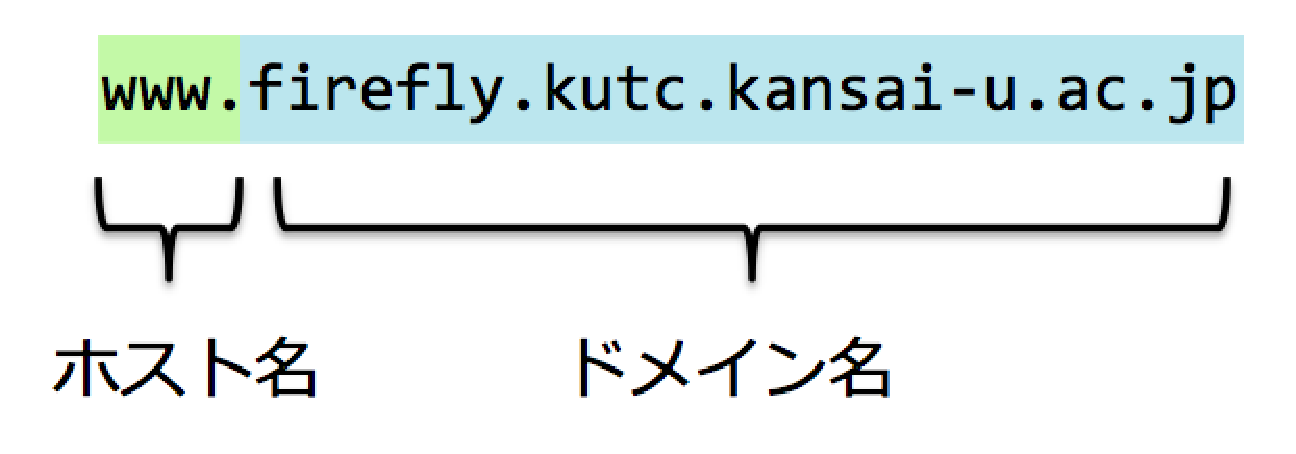
\includegraphics[width=100mm, bb=0 0 606 202]{hostdomain.eps} 
  \end{center}
  \caption{ドメイン名とホスト名}
  \label{fig:URI_hostdomain}
\end{figure}

FQDNは階層型の構造となっており,www.firefly.kutc.kansai-u.ac.jpは「日本(jp)の大学(ac)の関西大学(kansai-u)の高槻キャンパス(kutc)の小林ゼミ(firefly)のWebサーバ(www)」という意味である.

システムによっては末尾にドット(.)をつけることを表記のルールとしていることもあるので(例: www.firefly.kutc.kansai-u.ac.jp.)注意が必要である.

\subsection{nslookup}
nslookupはDNS問い合わせを手動で実施するためのコマンドである.任意のDNSサーバを指定して問い合わせを行うことも可能であり,DNSのトラブルシューティングでは非常に良く使用される.ネットワーク関連の基本的コマンドの一つである.\\

\fbox{nslookup [FQDNまたはIPアドレス] [任意のDNSサーバ名またはIPアドレス]}\\

一番基本的なnslookupの使い方は,引数にFQDNを指定してnslookupを起動することである.この使い方を『正引き』と呼び,FQDNに対応するIPアドレスがDNSサーバから取得される(図\ref{fig:nslookup1}).

\begin{figure}[htb]
  \begin{center}
    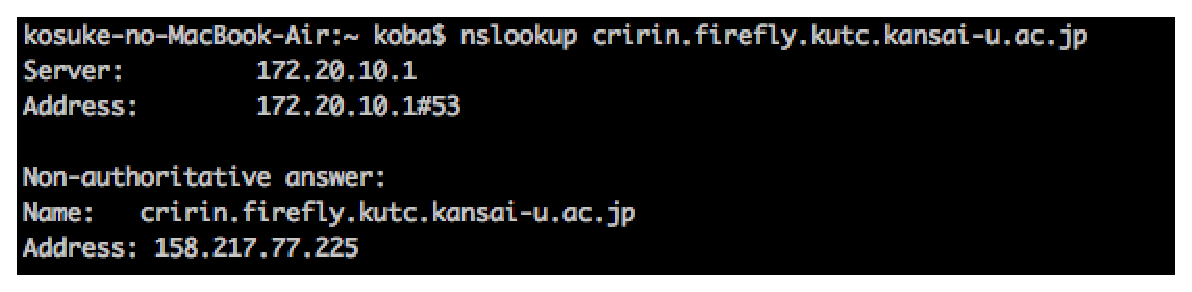
\includegraphics[width=150mm, bb=0 0 556 124]{nslookup1.eps} 
  \end{center}
  \caption{正引き}
  \label{fig:nslookup1}
\end{figure}

次によく使われるnslookupの使い方は,引数にIPアドレスを指定してnslookupを起動することである.この使い方を『逆引き』と呼び,IPアドレスに対応するFQDNがDNSサーバから取得される(図\ref{fig:nslookup2}).

\begin{figure}[htb]
  \begin{center}
    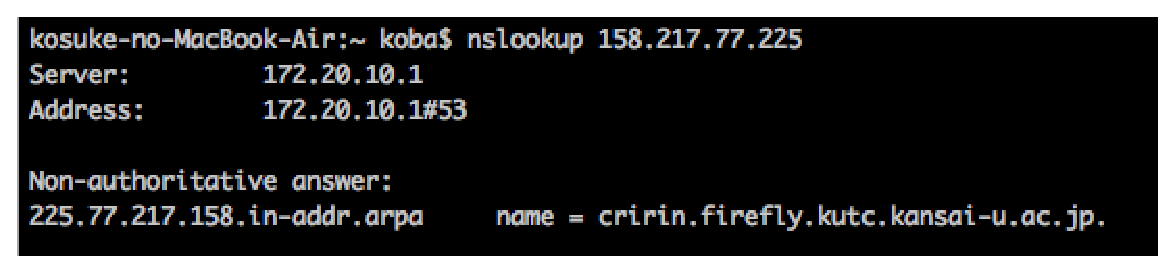
\includegraphics[width=150mm, bb=0 0 556 124]{nslookup2.eps} 
  \end{center}
  \caption{逆引き}
  \label{fig:nslookup2}
\end{figure}


\section{グローバルIPとプライベートIP}
%ネットワークのセグメントに有効.ファイアウォール
インターネットは接続先となる端末の所在を表すため,IPアドレスを用いているが,これはグローバルIPアドレスと呼ばれ世界中のネットワークに割り当てられる.
また,グローバルIPアドレスは住所と同じように世界中で重複することはなく,グローバルIPアドレスを割り当てられた端末に対しては,世界中から宛先として通信することが可能である.\par
ここでは,ネットワークの疎通を確認するpingコマンドを使用してグローバルIPアドレスへの通信を確かめる.
例として,小林研究室のグローバルIPアドレスである158.217.77.225に対して,pingコマンドを以下のように入力する.
\begin{screen}
\begin{Verbatim}[frame=single]
# ping 158.217.77.225
PING 158.217.77.225 (158.217.77.225): 56 data bytes
64 bytes from 158.217.77.225: icmp_seq=0 ttl=64 time=2.701 ms
64 bytes from 158.217.77.225: icmp_seq=1 ttl=64 time=3.708 ms
64 bytes from 158.217.77.225: icmp_seq=2 ttl=64 time=3.807 ms
                   :
※終了はctrl+c
\end{Verbatim}
\end{screen}
pingコマンドの結果を確認するとグローバルIPアドレスに対して疎通確認することができる.\par
グローバルIPアドレスは,前述した通り世界中で重複することはなく,IPアドレスの割り当て個数は32桁の2進数で約43億のパターンが存在する.
しかし,この個数は世界人口約70億人に対してインターネットを利用するデバイスが増加し続ける中でアドレスの枯渇が問題となっている.
そこで,企業や家庭などの限られたエリアごとにネットワークを構成し,このネットワーク内はグローバルIPアドレスの代わりに,プライベートIPアドレスというものを用いて割り当てを行っている.\par
プライベートIPアドレスは,企業や家庭内などのローカルなネットワーク内でのみ有効なアドレスであり,各ネットワークごとに所属する端末間で自由にアドレスを設定することができる.
これにより,各ネットワークごとに,プライベートIPアドレスを用いることでIPアドレスの割り当て個数を節約できる.
しかし,プライベートIPアドレスは自由に設定されるため,インターネット上からは直接参照することができず,また,異なるネットワークに属する端末同士も直接通信することができない.プライベートIPアドレスを使用したネットワーク通信については後述する.
\par
異なるネットワーク同士が通信できないことを確認してもらうため,pingコマンドを使用してプライベートIPアドレスから別のネットワークのプライベートIPアドレスに対して通信可能かどうかを確認する.
例として,現在接続されている関西大学のネットワーク(kuwifi)から,小林研究室のネットワークで運用されるサーバであるcririnのプライベートIPアドレス10.1.3.10に対して,pingコマンドを以下のように入力する.
\begin{screen}
\begin{Verbatim}[frame=single]
# ping 10.1.3.10
PING 10.1.3.10 (10.1.3.10): 56 data bytes
ping: sendto: No route to host
\end{Verbatim}
\end{screen}
結果を確認すると,宛先が見つからないため,プライベートIPアドレスには直接通信できないことが分かる.\par
上の例から異なるネットワークに属する端末同士は直接的に通信することができないことを確認したが,
これにより,IPアドレスの節約に加え,他のネットワークと隔離されていることを利用して,セキュリティの確保を実現することができる.
ネットワークを区切ることによる利点として,プライベートIPアドレスで構成されるネットワークは他のネットワークから切り離されるため,意図しないユーザからのアクセスを防ぐことができる.
さらに,ネットワークに侵入する通信をファイアウォールなどを用いてフィルタリングすることで,ネットワーク全体のセキュリティを確保することができる.
\begin{figure}[tbp]
 \begin{center}
  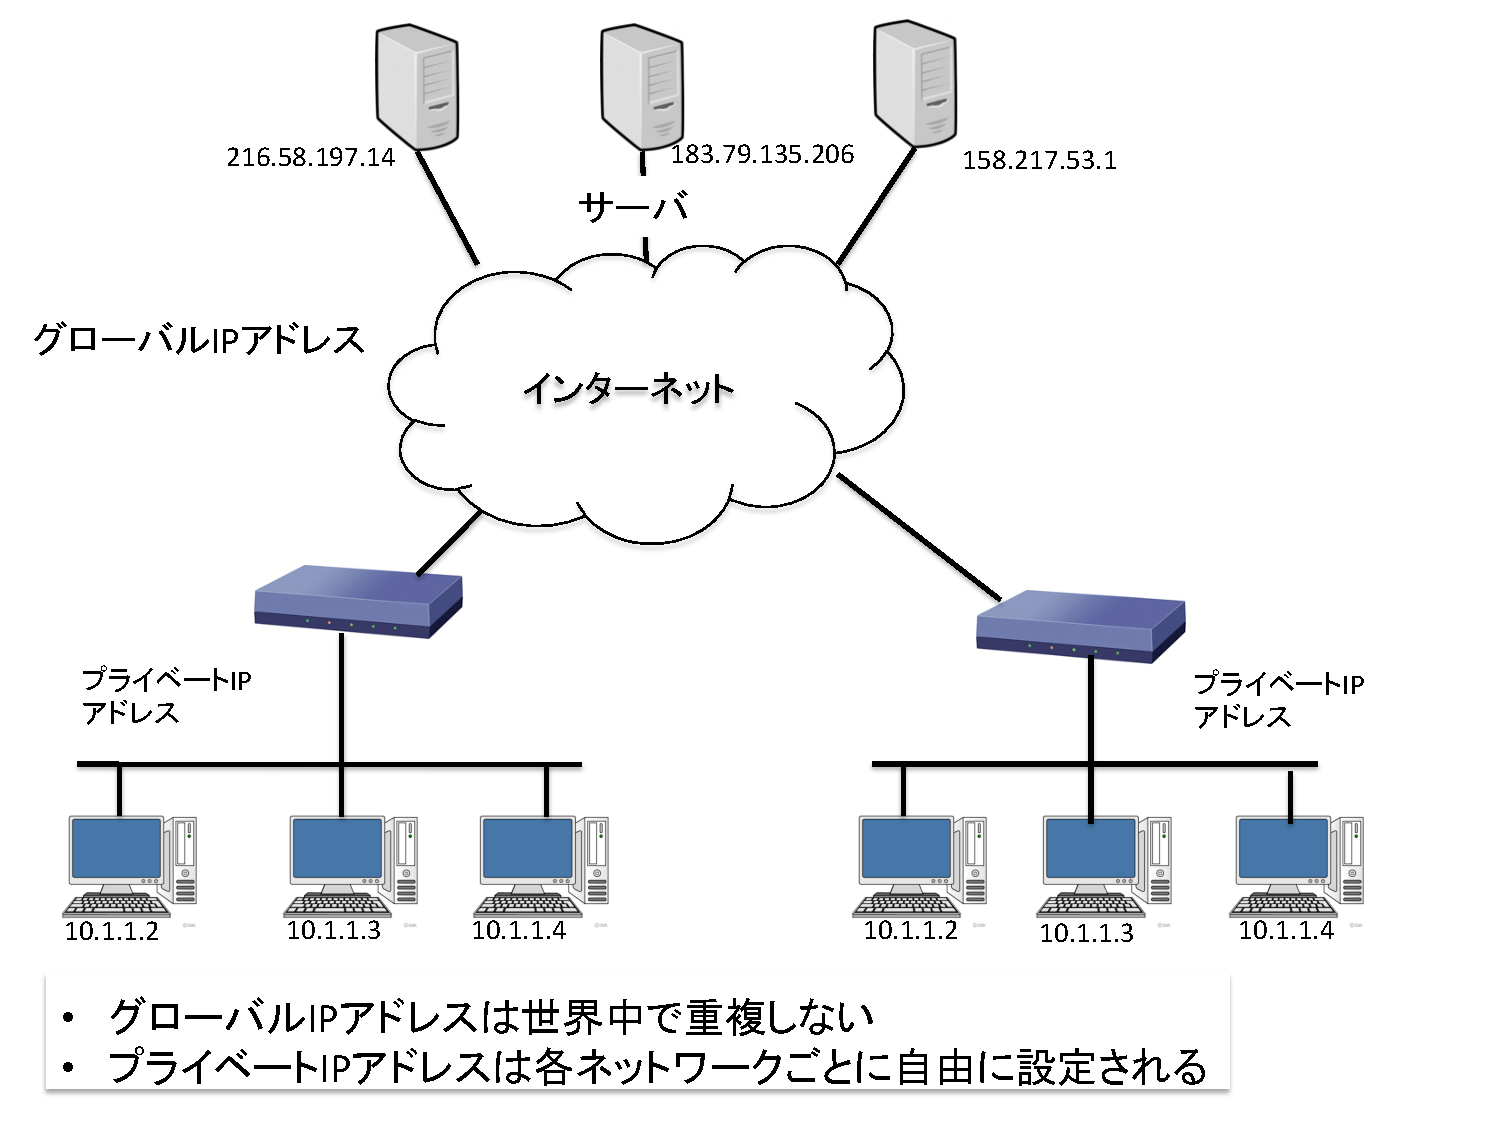
\includegraphics[width=14cm]{globalIP.pdf}
 \end{center}
 \caption{グローバルIPとプライベートIP}
 \label{glovalIP}
\end{figure}


\section{ルータ}
上の説明において,異なるネットワーク同士は直接通信できないと説明した.
しかし,異なるネットワークであるはずのグローバルIPアドレスに対してpingコマンドにより疎通を確認することができた.
また,私たちは日常においてインターネットを使用する際,無線LANなどから設定されたプライベートアドレスを用いて,インターネット上に存在するWebサイトなどのWebサービスを利用している.
これらのネットワークを越える通信はルータによって実現される.
ルータは異なるネットワーク間においてデータを中継する機器であり,インターネットに接続されるルータは外側にグローバルIPアドレス,内側にプライベートIPアドレスを割り当てられる.
このルータを用いることで,複数のネットワークで構成されるインターネット上においても,ルータが通信経路を中継することで目的の端末までデータを届けることができる(図\ref{router}).
こういった仕組みから,私たちはインターネット上の離れたネットワークに存在するサービスを利用することができる.
実際に通信経路を確認するため,例としてネットワーク経路を調べるtraceroute(tracert)コマンドを使用して関西大学のサーバまでの経路を確認する.

\begin{figure}[tbp]
 \begin{center}
  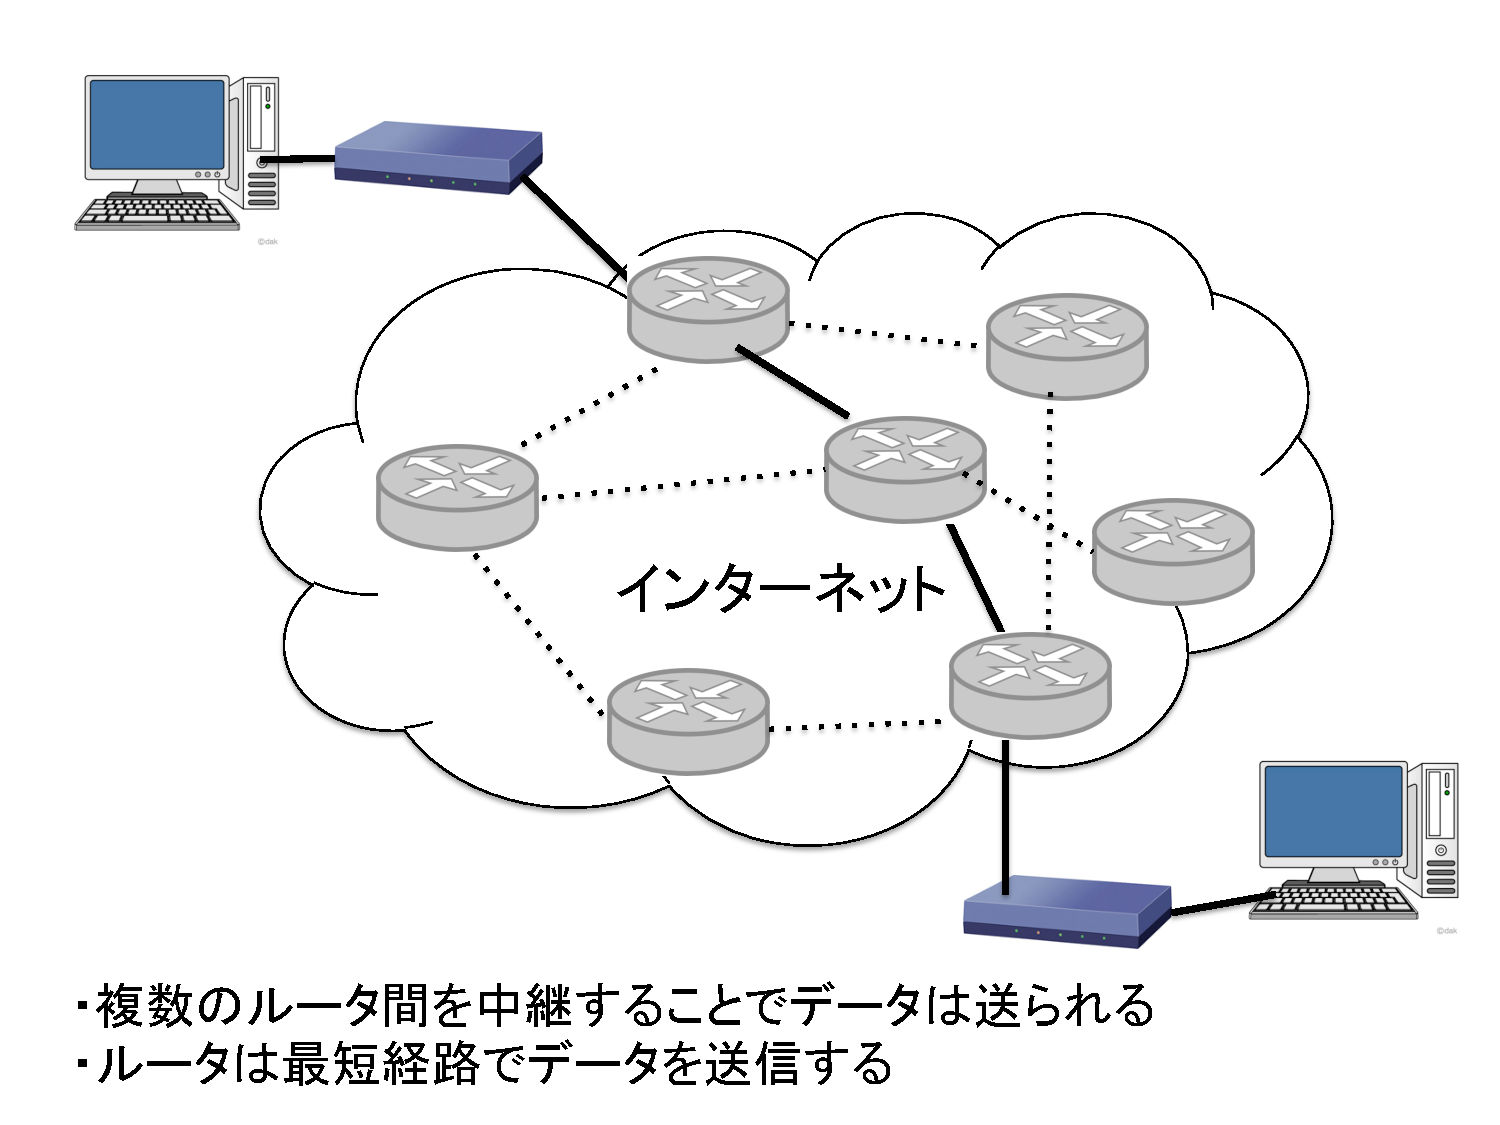
\includegraphics[width=10cm]{routing.pdf}
 \end{center}
 \caption{ルータによるデータの転送}
 \label{router}
\end{figure}
\newpage
Macは以下のコマンドを入力する.
\begin{screen}
\begin{verbatim}
# traceroute sh.edu.kutc.kansai-u.ac.jp
traceroute to sh.edu.kutc.kansai-u.ac.jp (158.217.53.13), 64 hops max, 52 
byte packets
 1  witccnt003.itc.kansai-u.ac.jp (172.29.70.203)  2.003 ms  0.975 ms  0.960 
 ms
 2  172.29.143.254 (172.29.143.254)  2.111 ms  2.154 ms  2.371 ms
 3  158.217.103.254 (158.217.103.254)  3.114 ms  3.504 ms  2.996 ms
 4  172.17.5.240 (172.17.5.240)  4.834 ms  4.463 ms  4.421 ms
 5  158.217.4.1 (158.217.4.1)  4.249 ms  3.509 ms  3.742 ms
 6  sh.edu.kutc.kansai-u.ac.jp (158.217.53.13)  2.920 ms !Z  2.992 ms !Z  
 4.961 ms
 \end{verbatim}
\end{screen}

windowsは以下のコマンドを入力する.
%結果を変更すること
\begin{screen}
\begin{Verbatim}[frame=single]
> tracert sh.edu.kutc.kansai-u.ac.jp
sh.edu.kutc.kansai-u.ac.jp[158.217.53.13]へのルートをトレースしています
経由するホップ数は最大30です:
1  1ms 3ms   2ms  witccnt003.itc.kansai-u.ac.jp [172.29.70.203]
2  2ms  5ms  1ms  172.29.143.254
3  3ms  2ms  3ms  158.217.103.254
4  9ms  4ms  4ms  172.17.5.240
5  3ms  3ms  4ms  158.217.4.1
6  3ms  3ms  4ms  sh.edu.kutc.kansai-u.ac.jp [158.217.53.13]
トレースを完了しました。
\end{Verbatim}
\end{screen}
traceroute(tracert)コマンドの結果から,宛先までの経路が中継されていることが確認できる.

\section{ドメイン情報}
前の説明で宛先に関西大学のドメインを指定したように,インターネット上のサービスを利用する際はIPアドレスを指定するより,アドレスに対応付けられたドメイン名を使用することが一般的である.
また,このドメインについては,whoisサービスにより所有先の情報を調べることができる.
whoisサービスは,登録者情報,ネームサーバホスト情報,担当者情報などを確認することができる.
また,代表的なものとして,ANSI(\verb| http://whois.jprs.jp/ |)やJPRS(\verb|http://whois.ansi.co.jp/|)などがWebサービスを提供している.
(Unix系OSの場合,whoisコマンドを使用することでも検索することができる.)\par
ドメイン情報を調べるwhoisサービスの検索方法を説明する.
まず,インターネットブラウザからJPRSを検索し,検索結果からJPRS WHOIS /JPRSを選択する(図\ref{whois1}).
次に,ドメイン名登録情報検索に検索キーワードとして,関西大学のドメインであるkansai-u.ac.jpを入力し,検索ボタンを押下する(図\ref{whois2}).
検索結果からドメインの登録情報を確認することができる(図\ref{whois3}).

\begin{figure}[htbp]
 \begin{center}
  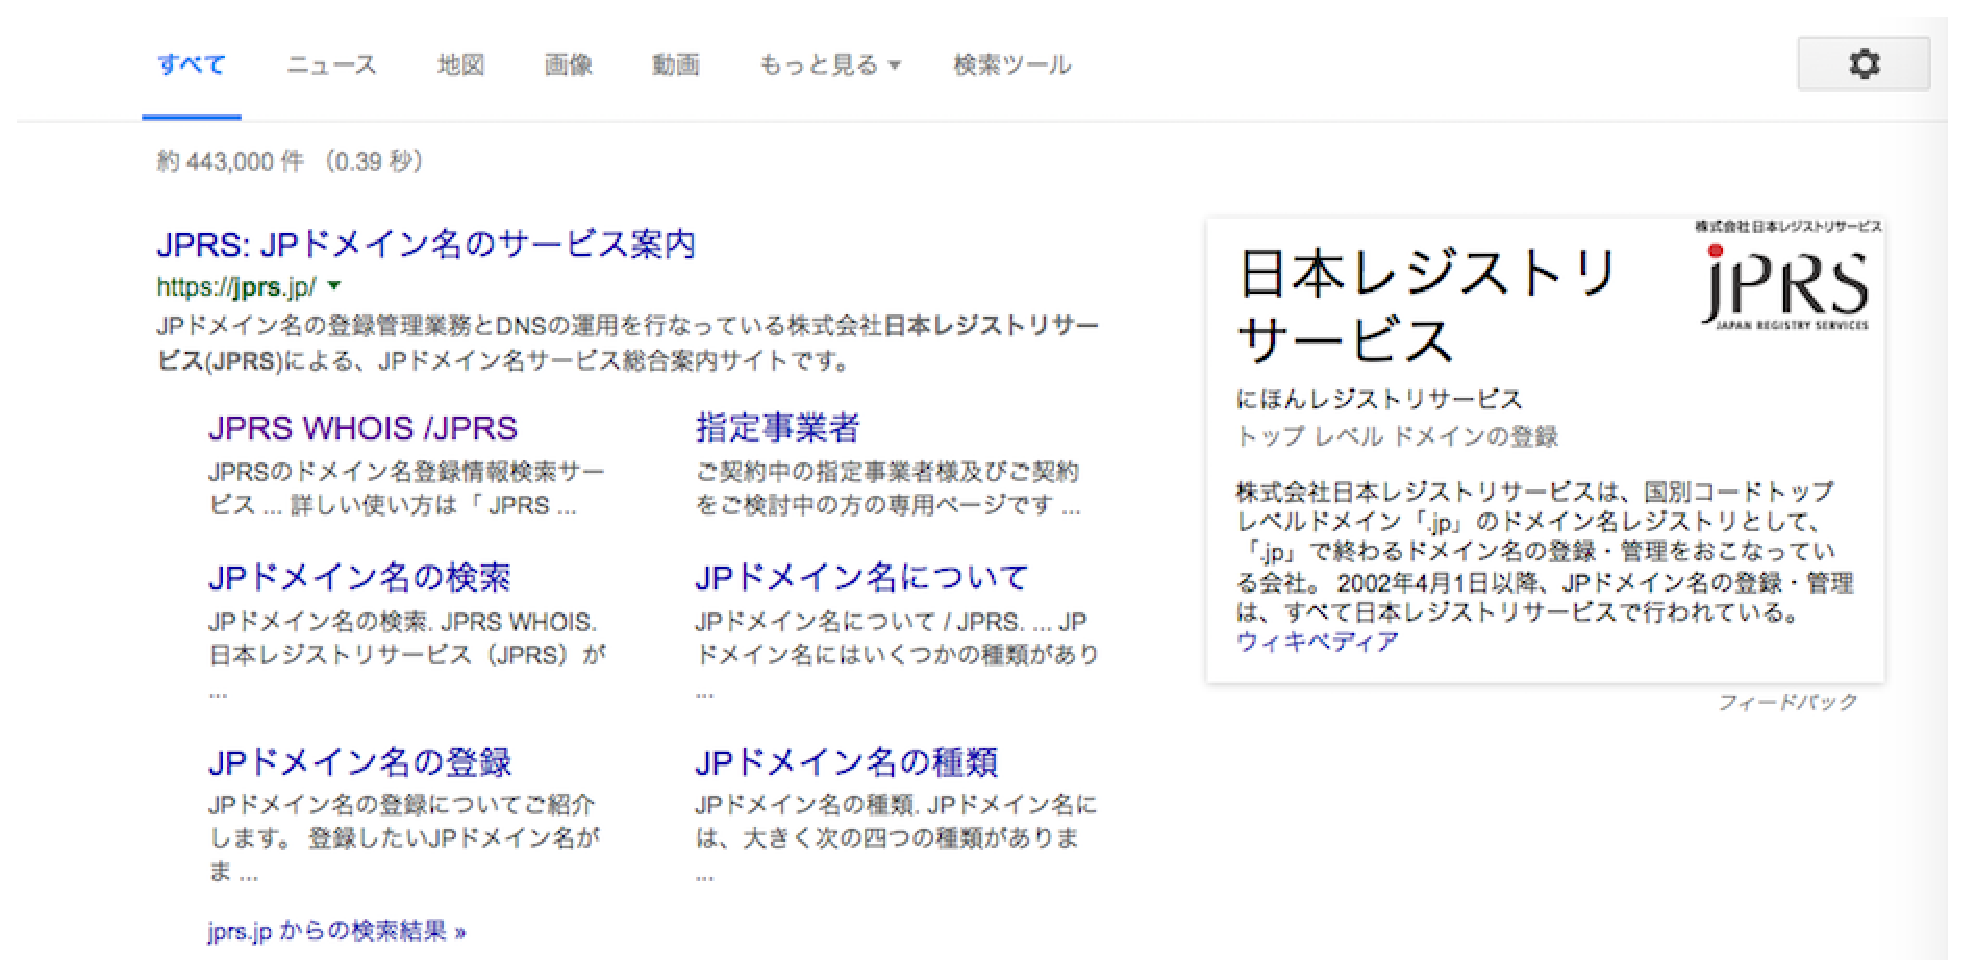
\includegraphics[width=15cm]{whois1.eps}
 \end{center}
 \caption{JPRSの検索}
 \label{whois1}
\end{figure}


\begin{figure}[htbp]
 \begin{center}
  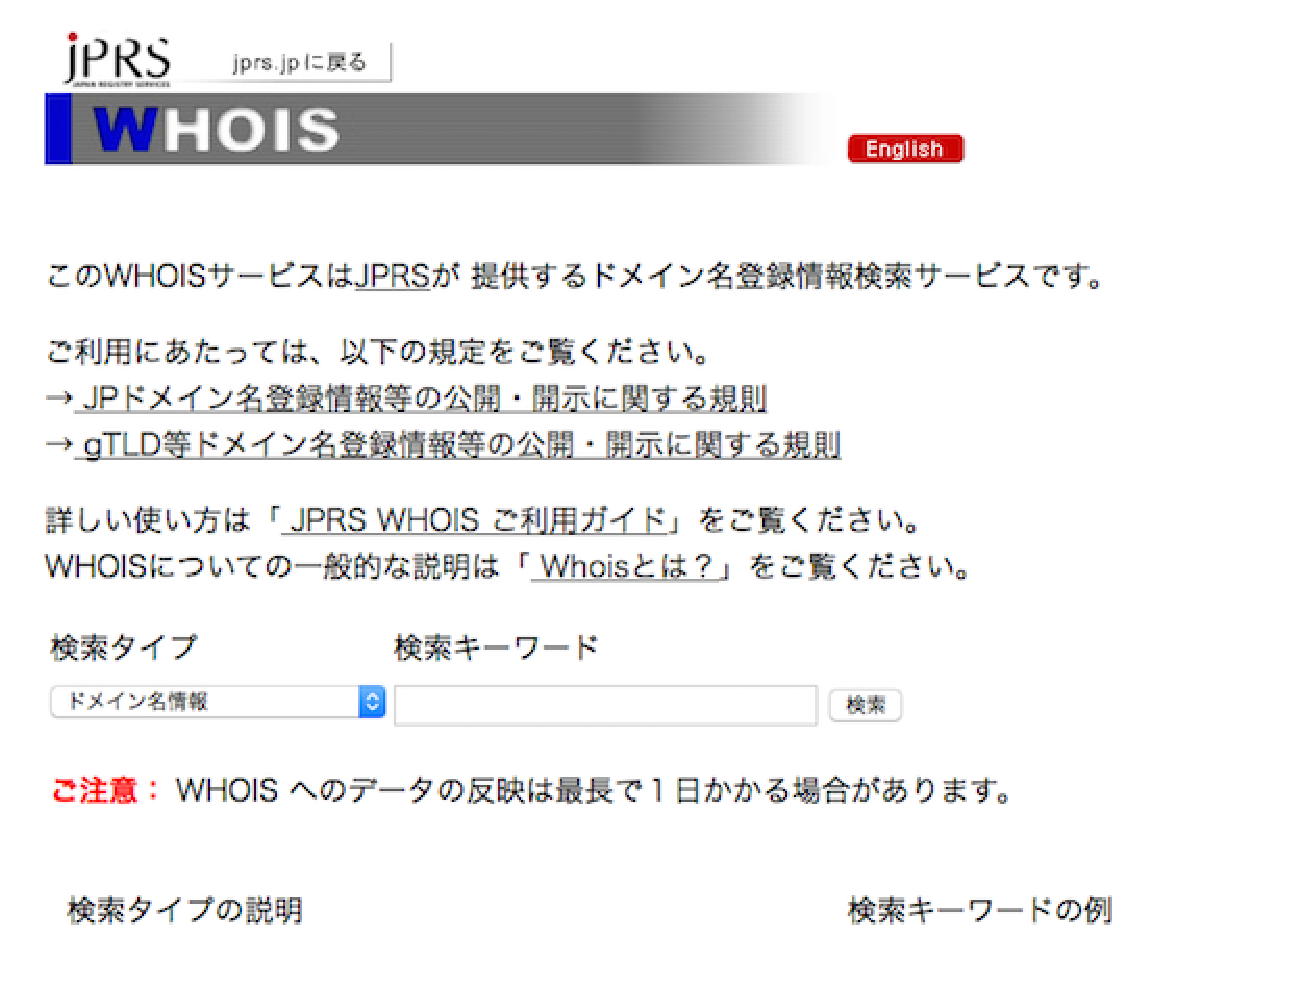
\includegraphics[width=12cm]{whois2.eps}
 \end{center}
 \caption{ドメイン名登録情報検索}
 \label{whois2}
\end{figure}

\begin{figure}[htbp]
 \begin{center}
  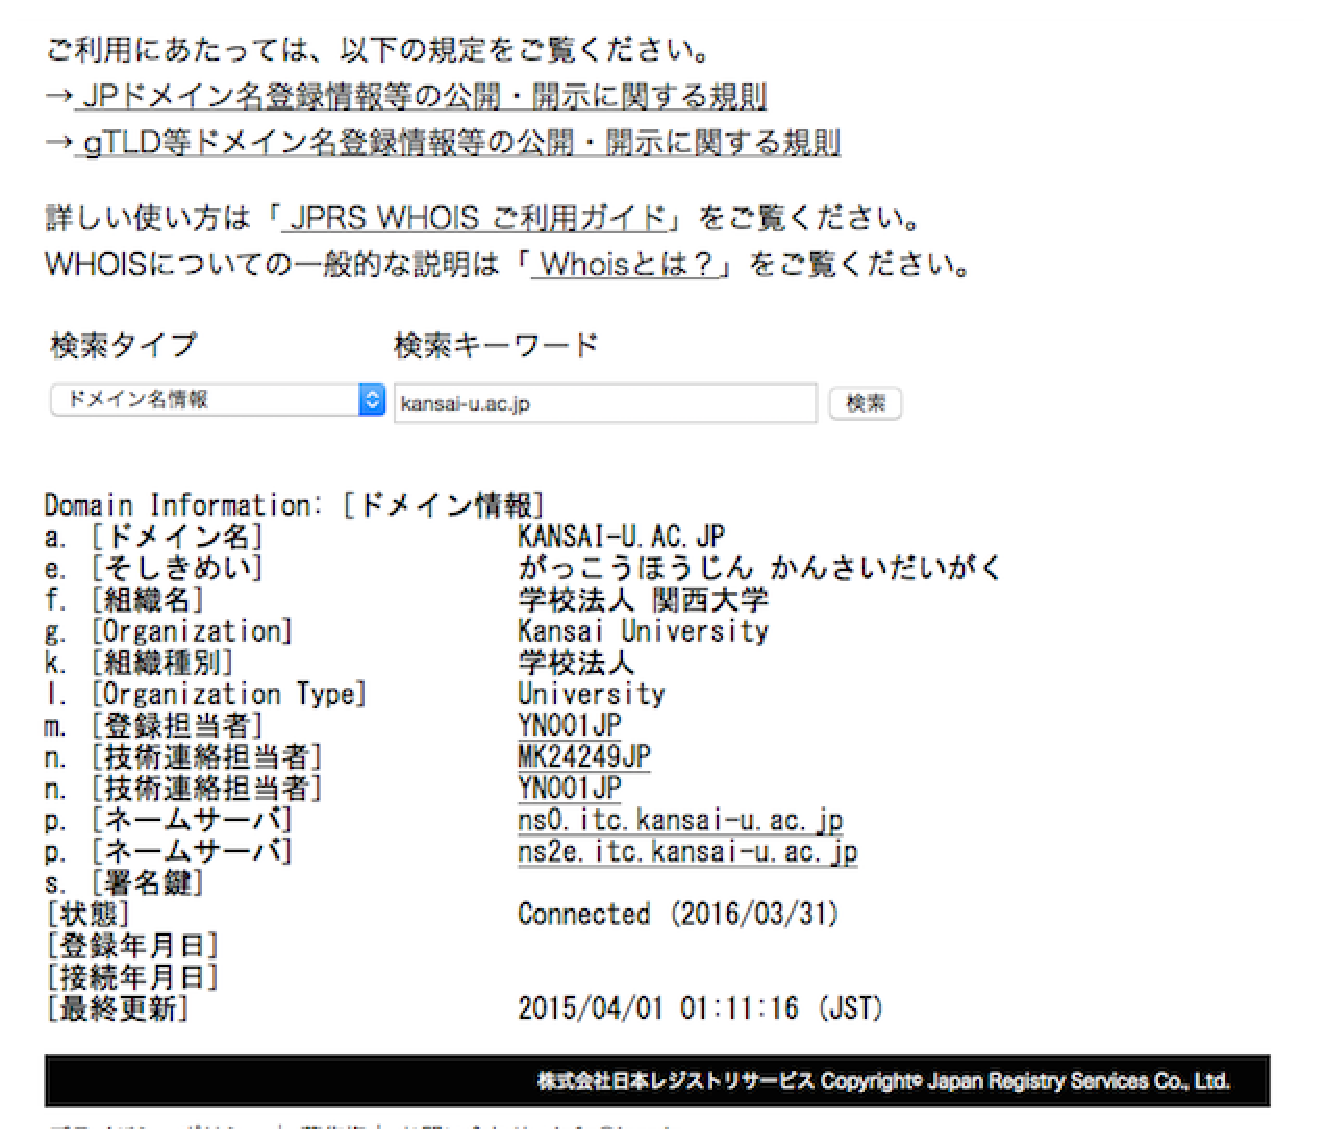
\includegraphics[width=13cm]{whois3.eps}
 \end{center}
 \caption{ドメイン情報結果}
 \label{whois3}
\end{figure}

\newpage

\section{NATとNAPT}
%グローバルとプライベートで通信を行う仕組み
ここでは,ルータの機能としてグローバルIPアドレスとプライベートIPアドレスの通信について説明する.\par
前述のIPアドレス枯渇問題から,プライベートIPアドレスの割り当てを説明したが,
グローバルIPアドレスが振られるインターネット側からは,プライベートIPアドレスを認識することはできない.
そこで,グローバルネットワークとプライベートネットワークの通信を可能にするため,ルータのNAT(Network Address Translation)機能を用いている.
インターネットに繋がるルータには,外側にグローバルIPアドレス,内側にプライベートIPアドレスを割り当てられているが,
NATはこのグローバルIPアドレスとプライベートIPアドレスの変換を行う.\par
NATの仕組みとして,プライベートIPアドレスが割り振られた端末が,インターネット上のグローバルIPアドレスと通信を行う場合について説明する.\par
まず,プライベートIPアドレスから送信があった場合,ルータは送信元となるプライベートIPアドレスはルータの外側にあるグローバルIPアドレスに変換する.そして,送信元がグローバルIPアドレスとなったデータは,インターネット上の宛先へと送信される.
次に,インターネット上から送信元に対して返信があった場合は,変換された送信元であるルータの外側のアドレスに対して返信される.そして,返信を受け取ったルータは送信先を本来の送信元であるプライベートIPアドレスに転送することで,インターネット上との通信を可能にする.\par
このように,ルータが中継となってアドレスを変換することで,プライベートIPアドレスとグローバルIPアドレス間で通信を行うことを可能にする(図\ref{nat}).

しかし,NATでのアドレス変換は一つのグローバルIPアドレスに対して,一つのプライベートIPアドレスを対応づけるため,
グローバル側との通信は一つの端末のみに限られてしまう.
そこで,NAT機能の拡張としてNAPT(Network Address Port Translation)の機能が用いられる.
NAPTは,一つの端末しか接続できない問題に対応するため,ポート番号を用いる.
ポート番号はサーバが提供するサービスを識別する番号である.
このポート番号を端末ごとに割り当て,番号をもとに宛先の端末を識別することで,ポート番号を利用して複数の端末により通信を行うことが可能となる.
\begin{figure}[htbp]
 \begin{center}
 %\vspace{-1cm}
  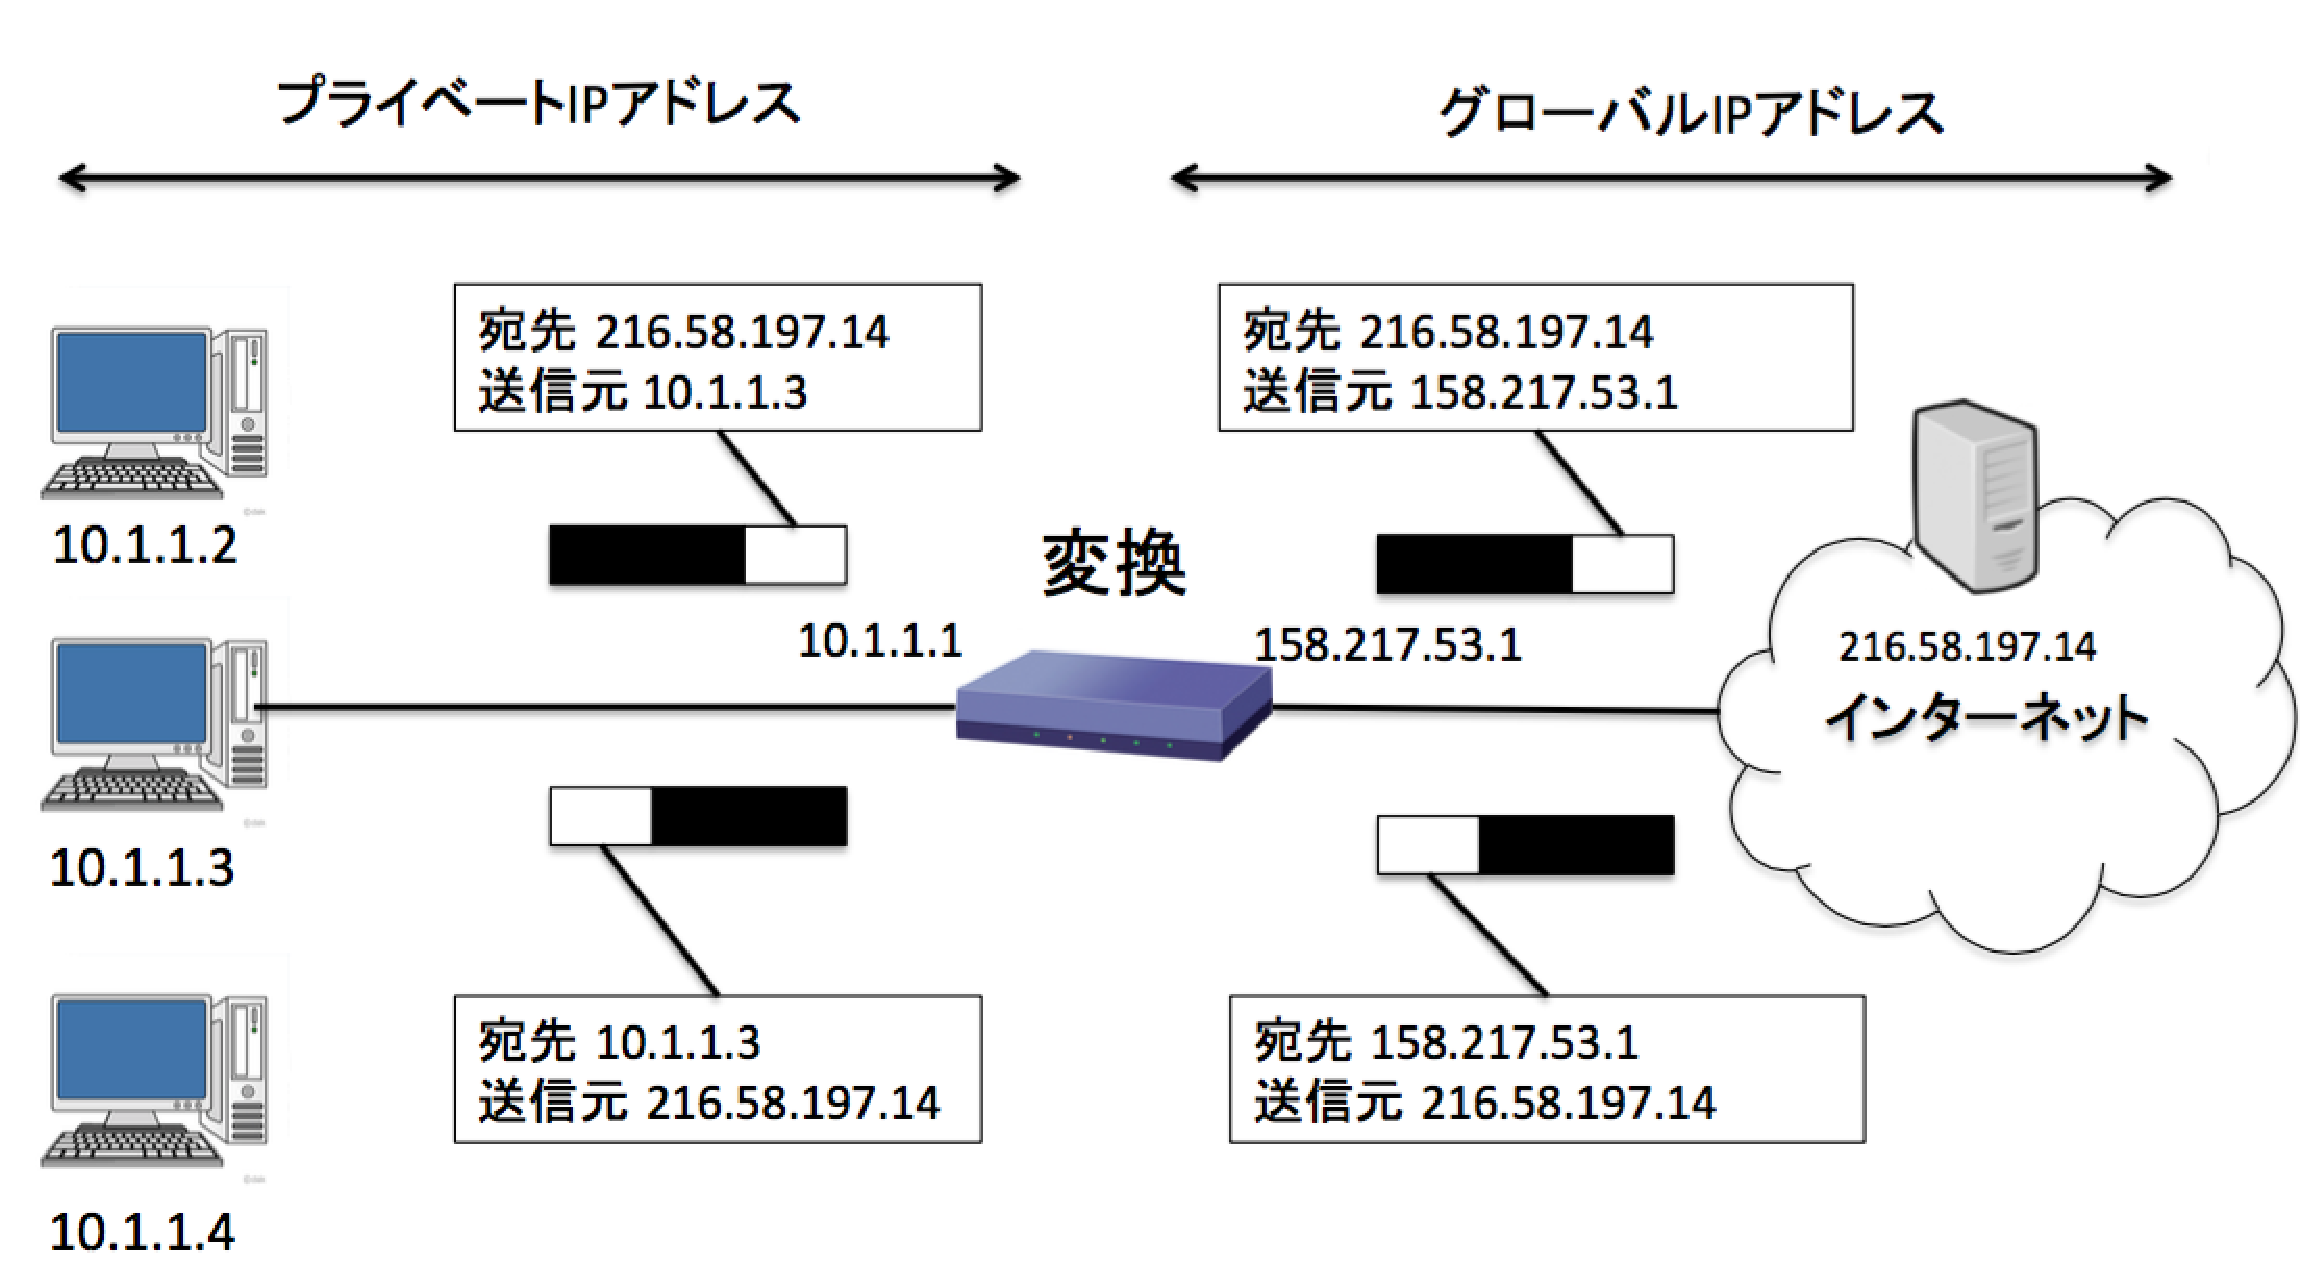
\includegraphics[width=14cm]{nat.eps}
 \end{center}
 \caption{NATによるアドレス変換}
 \label{nat}
\end{figure}

\subsection{DHCP}
ここまで,プライベートIPアドレスを利用した技術の説明をした.
プライベートIPアドレスの使用に伴い,ネットワークで管理される端末数も増加し,IPアドレスの管理も大変になる.
しかし,日常生活で利用する際にIPアドレスを設定する機会はほとんどない.
多くの場合,実際のIPアドレスの設定はDHCP(Dynamic Host Configuration Protocol)により行われる.
また,設定機能を持った機器をDHCPサーバと呼ぶ.
これは,IPアドレスやDNSなどのネットワーク情報を持っており,ネットワークに接続した端末に対して設定情報を提供する.
また,端末がネットワークから離脱するとDHCPリソースを更新する.
このようにDHCPは,IPアドレスの割り当てなど,ネットワーク情報を自動的に管理することができる.

%VPNについて
\section{VPN(Virtual Private Network)}
自宅など,外部のネットワークからゼミ内のプライベートIPアドレスが割り振られているマシンなどを操作する場合はネットワークが異なるため,直接的に利用することはできない.
そこでVPNという技術を用いることで,異なるネットワーク同士を仮想的に同一のネットワークに属しているように見せかけ,
異なるネットワークの端末と通信することができるようになる.\par
VPNによる通信の仕組みとして,トンネリングによりネットワークを繋いでいる.
トンネリングでは,もとの通信内容にヘッダが加えられ,加えられたヘッダにより通信内容はカプセル化される.このカプセル化を用いることで接続元でカプセル化を行い,接続先でカプセル化を解除し通信内容を取り出すことで,ネットワーク同士をトンネルで繋いだように見立てて使用することが可能となる.
さらに,データをカプセル化する際は,データを暗号化することで安全にネットワークを越えて通信することが可能となる(図\ref{vpn}).
VPNで利用されるプロトコルには,IPsec/PPTP/L2TP/L2F/MPLSなどがある.
\begin{figure}[htbp]
 \begin{center}
  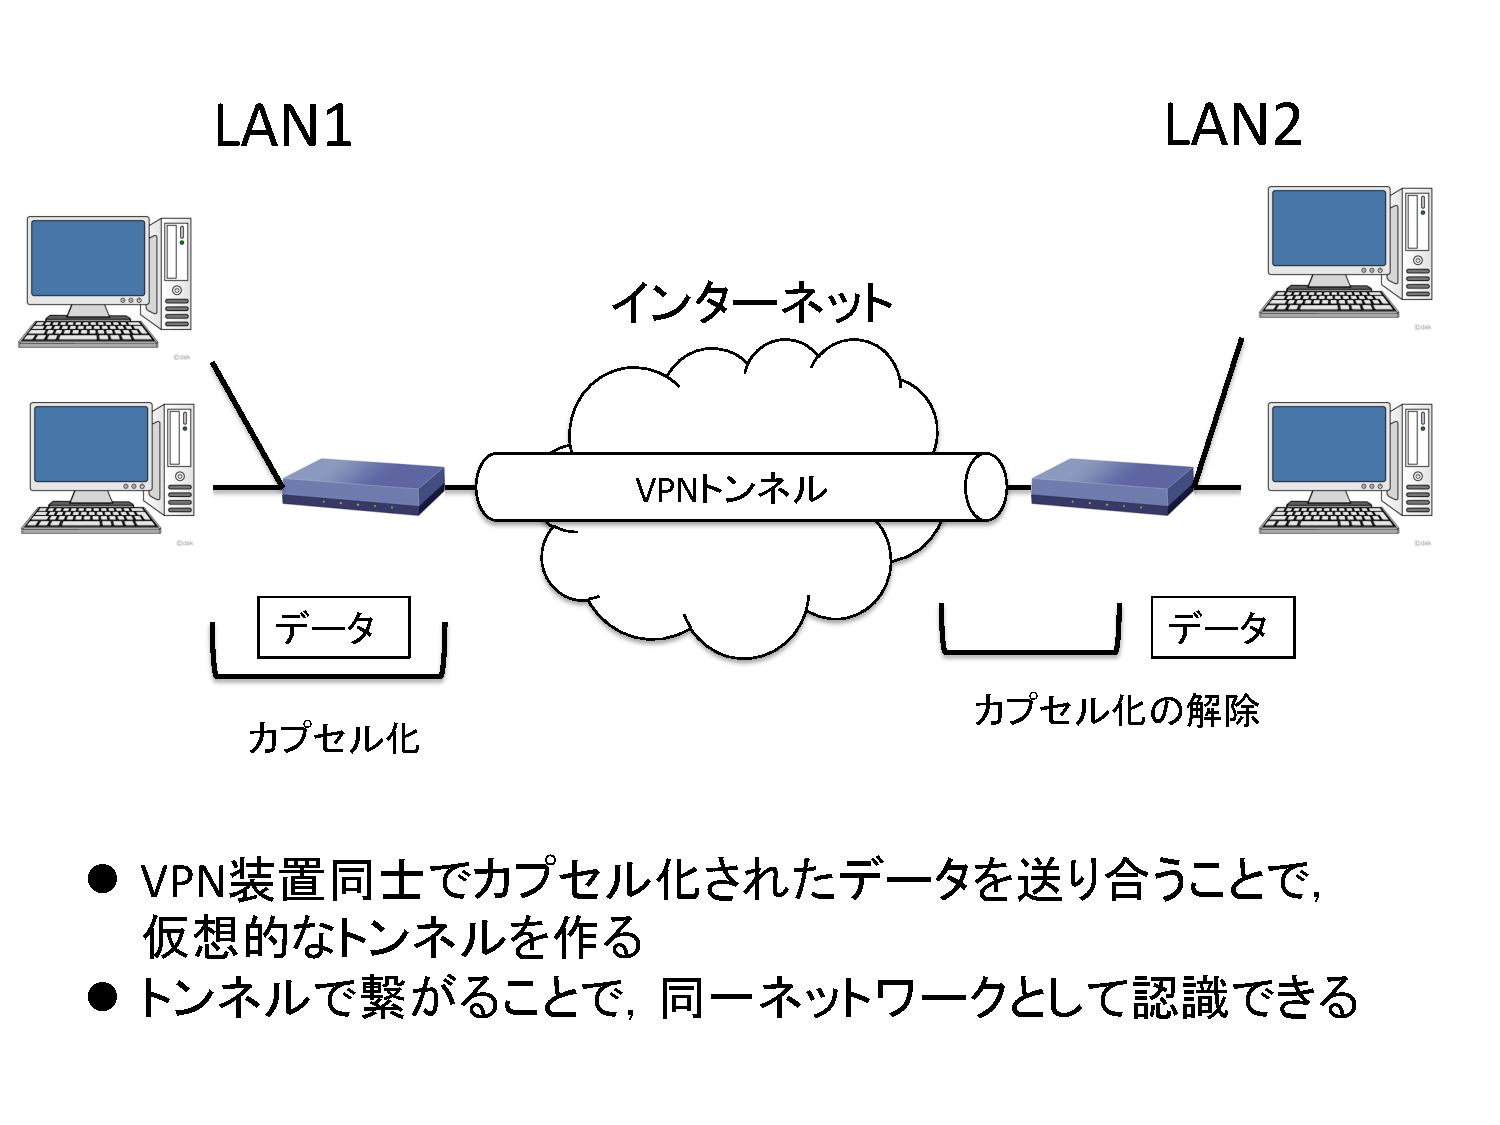
\includegraphics[width=13cm]{vpn.pdf}
 \end{center}
 \caption{VPNの概要}
 \label{vpn}
\end{figure}

\newpage

\subsection{小林ゼミのVPN}
小林ゼミのVPN環境において利用可能なプロトコルはL2TP Over IPSecとPPTPがある.
Macはいずれのプロトコルも利用することが可能である.ただし,L2TP Over IPSecはPPTP
よりもセキュアなため前者の使用を推奨する.はじめに,VPNの設定に必要な情報を表\ref{servers}に示す.
サーバアドレスはcririn.firefly.kutc.kansai-u.ac.jpと同じ158.217.77.225を使用する.
アカウント名とパスワードはXoopsにログインする時と同じものを使用する.共有シークレットは口頭で伝える.
\begin{table}[htbp]
\begin{center}
\caption{VPN設定に必要な情報}
\label{servers}
\begin{tabular}{| l | l |c|}
	\hline
	項目 & 値  \\ \hline
	サーバアドレス & 158.217.77.225 \\ 
	 アカウント名 & Xoopsで使用するアカウント名 \\
  	パスワード & Xoopsで使用するパスワード \\ 
	 共有シークレット & ****** \\ \hline
\end{tabular}
\end{center}
\end{table}
\subsection{VPNの設定(Macの場合)}
システム環境設定からネットワークを開く(図\ref{Mvpn1}).次に+から新しいサービスを作成する.
新たに表示されたウィンドウでインタフェースをVPN,VPNタイプをL2TP Over IPSecかPPTPを選択,
サービス名は任意に入力して,作成を押す(図\ref{Mvpn2}).
新しいサービスが作成されたので,そのサービスを選択した状態で設定を入力する.構成はデフォルト,サーバアドレスは158.217.77.225,
アカウント名を入力する.次に認証設定を押す.
ここでL2TP over IPSecによるVPN構成の場合は,ユーザ認証でパスワード,コンピュータ認証で共有シークレットを入力する(図\ref{Mvpn4}).
PPTPによるVPN構成の場合はパスワードを入力する.
さらにPPTPの暗号化は自動(128ビットまたは40ビット)にする.
以上全ての項目を入力して,適応と接続を行う.またメニューバーにVPNの状況を表示をチェックすることで接続状態や接続時間が表示される.
これはVPN接続のショートカット機能も有しているのでチェックすることを推奨する(図\ref{Mvpn3}).
\begin{figure}[htbp]
 \begin{center}
  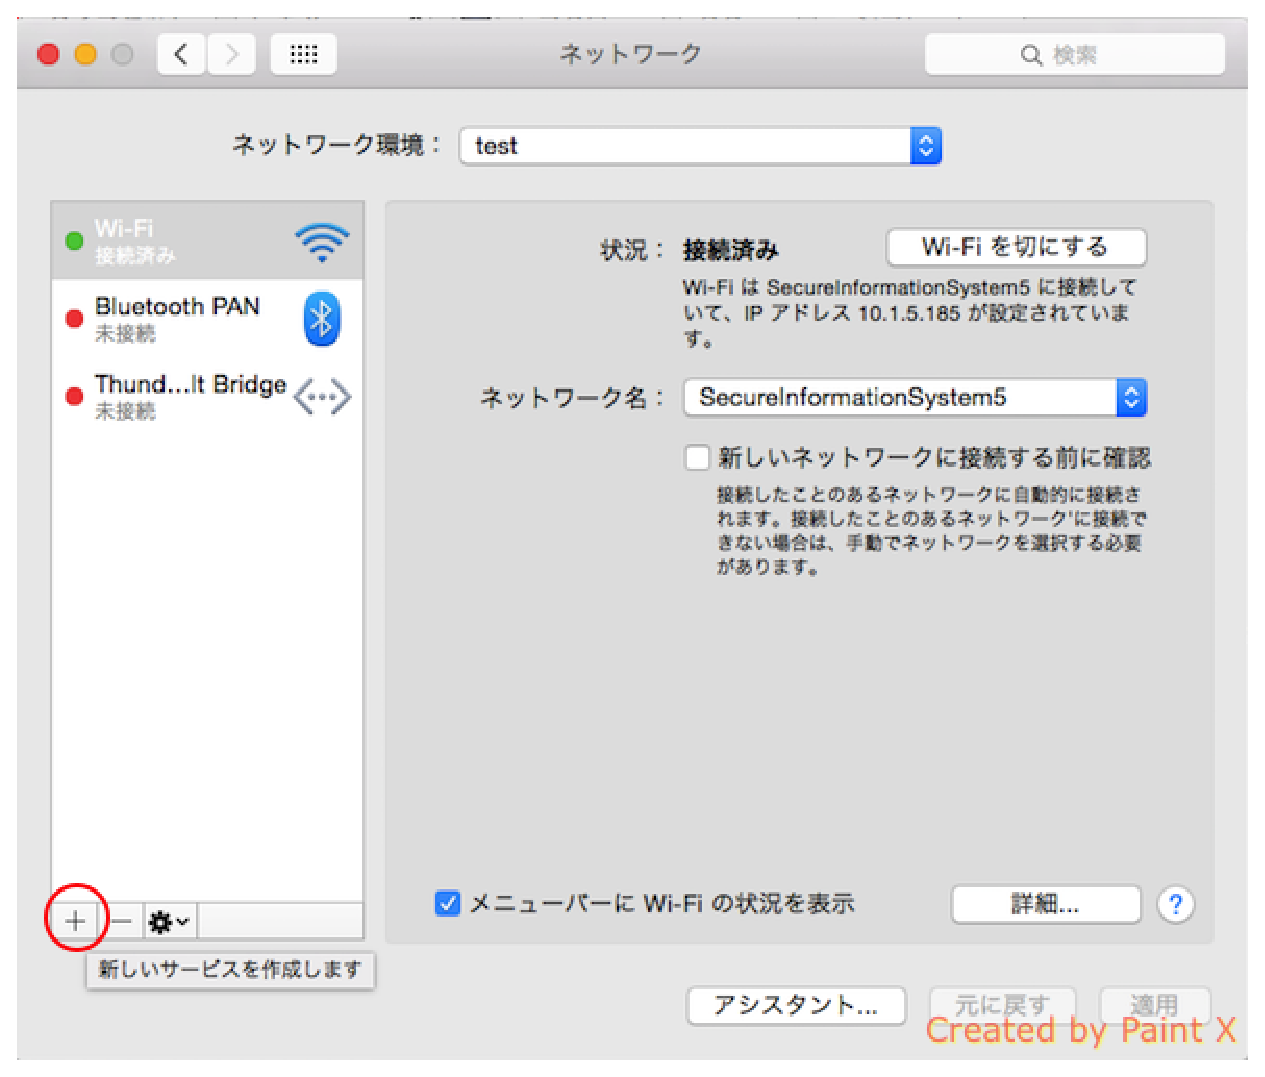
\includegraphics[width=13cm]{vpn1-mac.eps}
 \end{center}
 \caption{ネットワーク設定}
 \label{Mvpn1}
\end{figure}

\begin{figure}[htbp]
 \begin{center}
  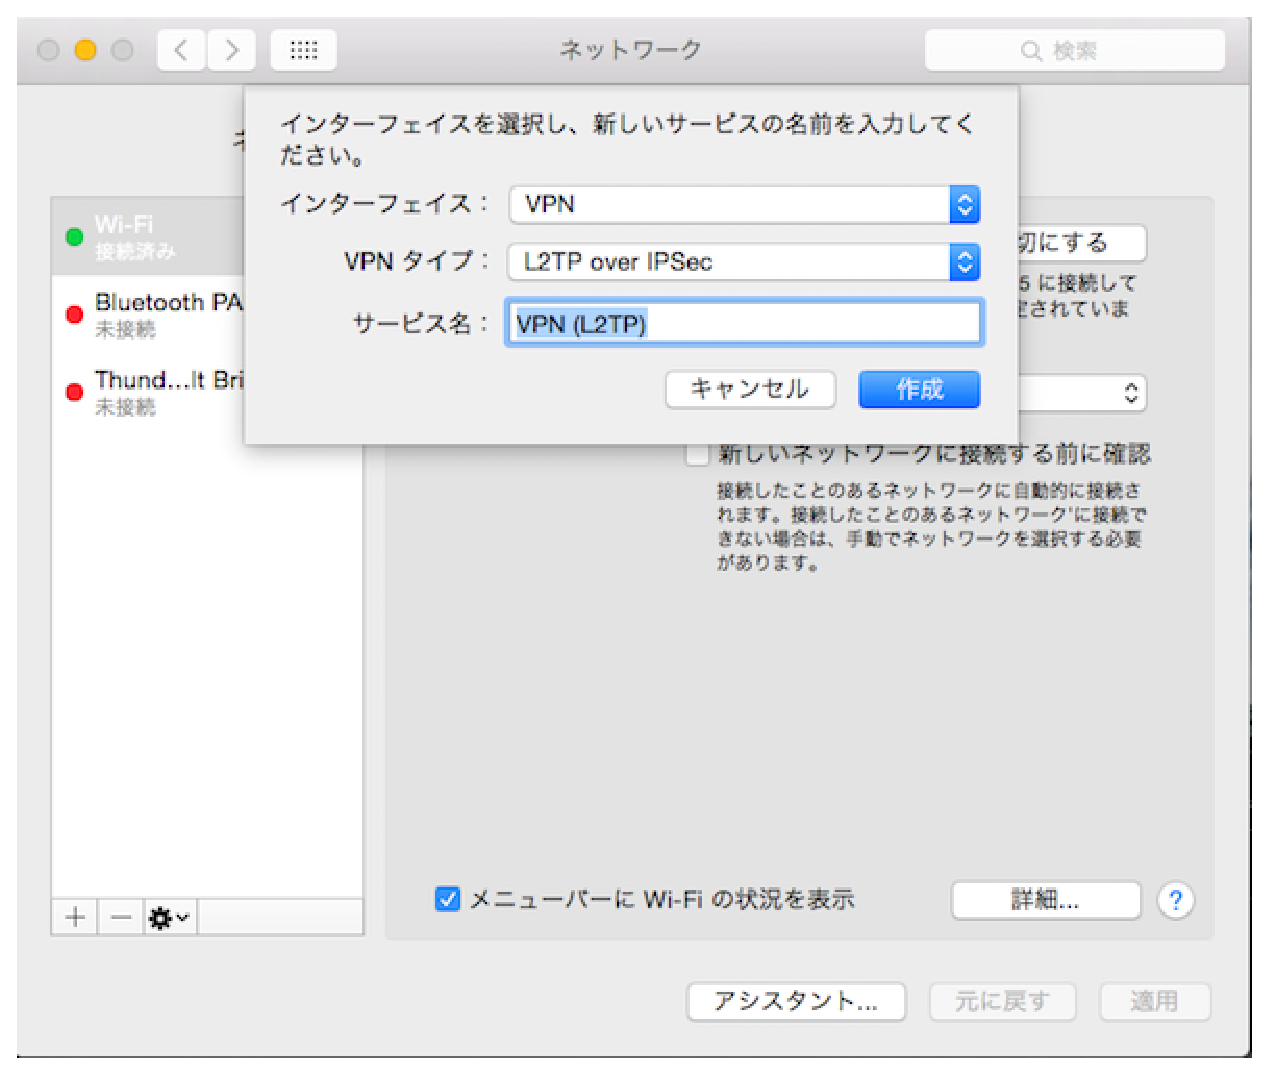
\includegraphics[width=13cm]{vpn2-mac.eps}
 \end{center}
 \caption{vpnサービスの作成}
 \label{Mvpn2}
\end{figure}

\begin{figure}[htbp]
 \begin{center}
  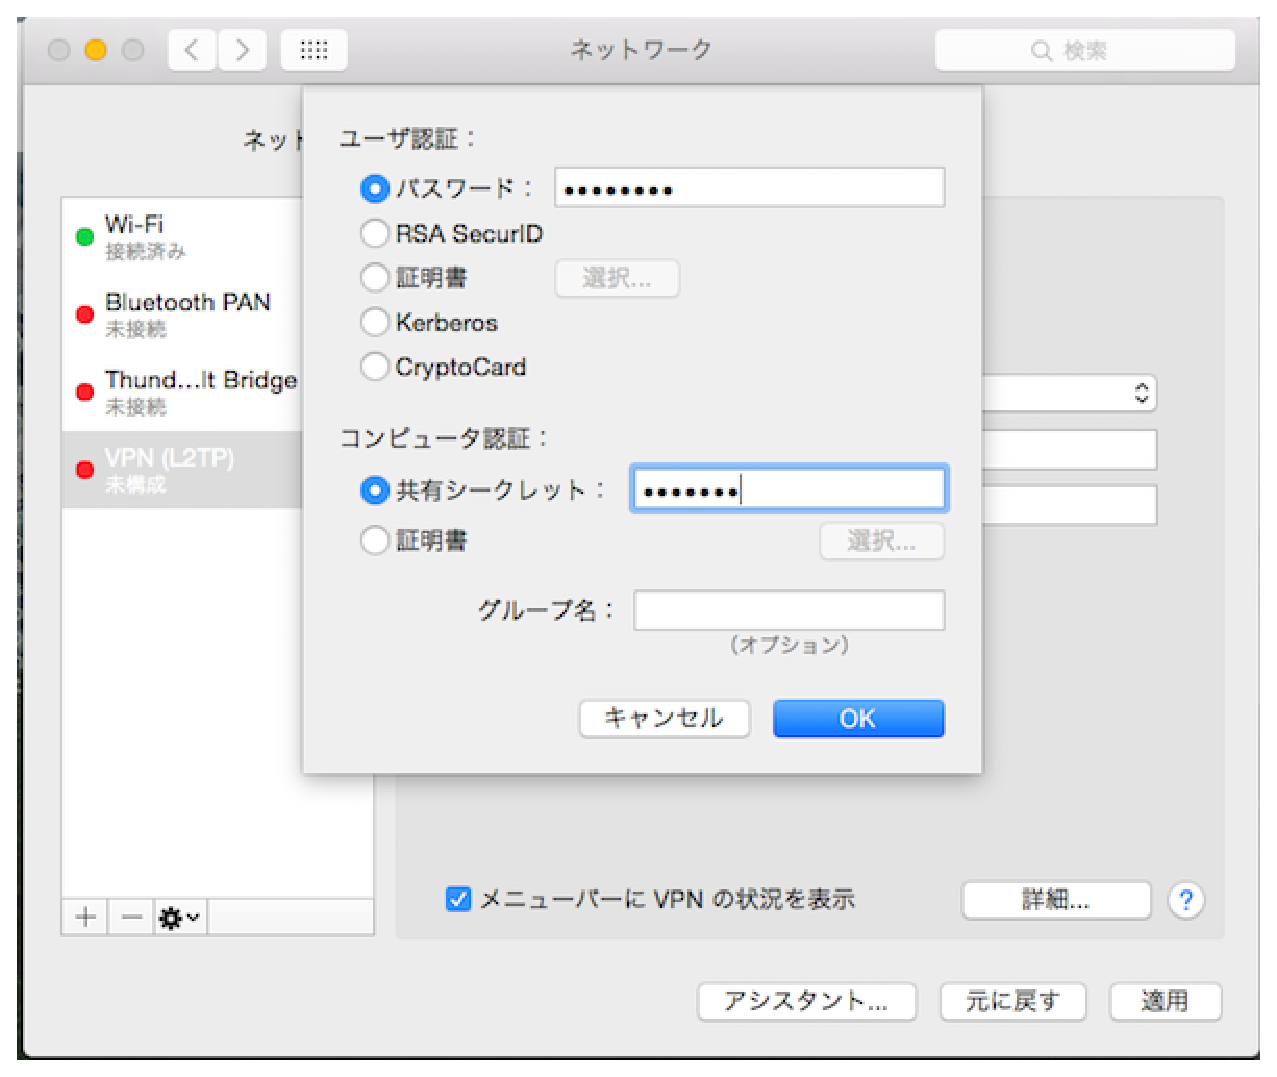
\includegraphics[width=13cm]{vpn4-mac.eps}
 \end{center}
 \caption{ L2TP Over IPSecの認証設定}
 \label{Mvpn4}
\end{figure}

\begin{figure}[htbp]
 \begin{center}
  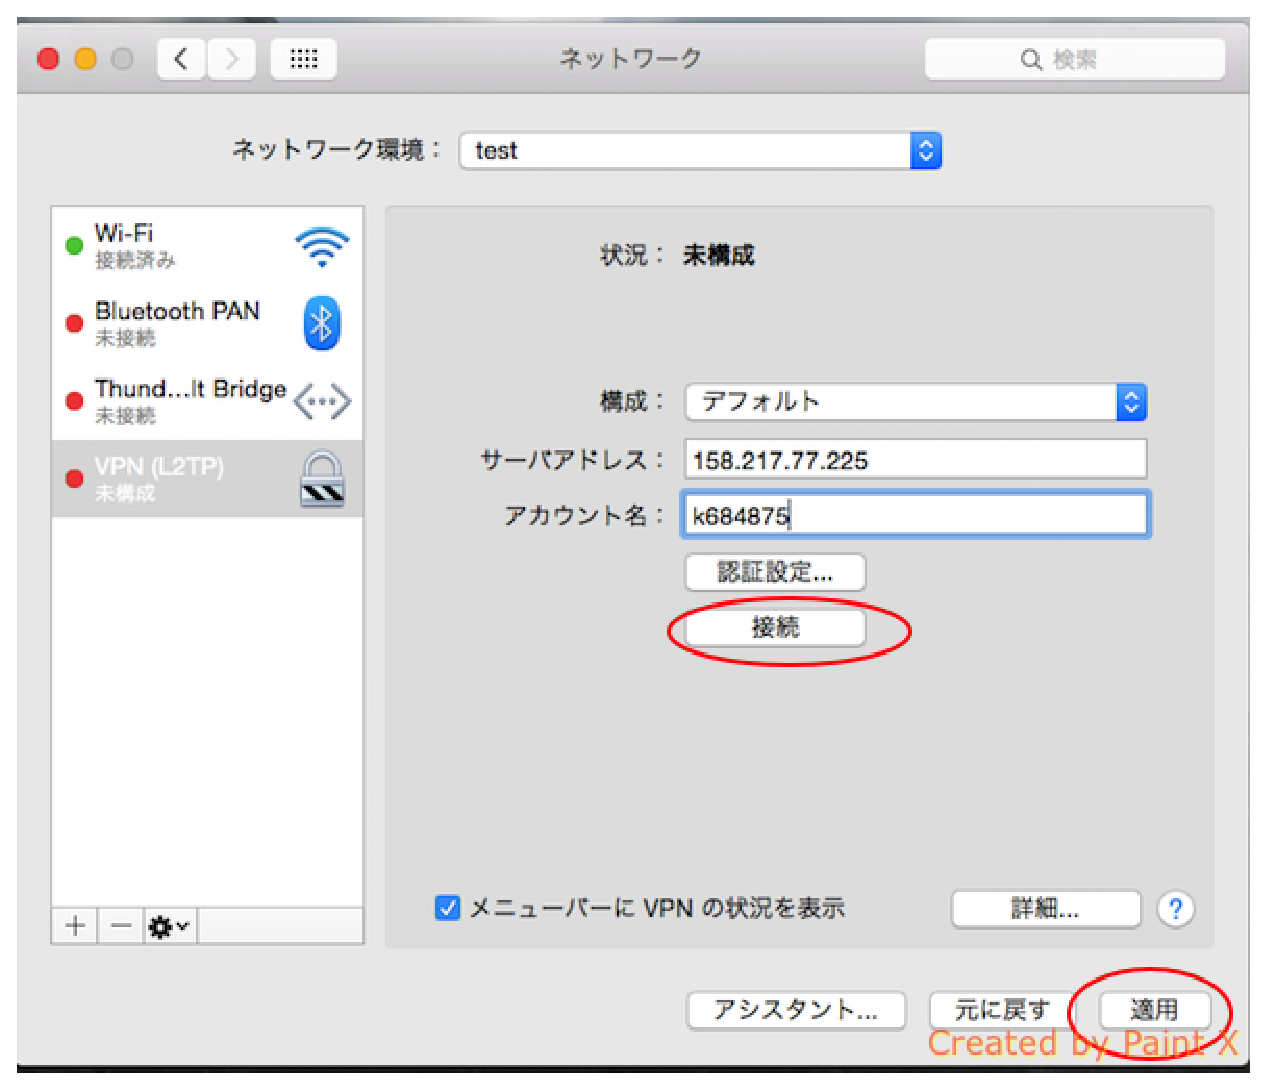
\includegraphics[width=13cm]{vpn3-mac.eps}
 \end{center}
 \caption{VPNの適応と接続}
 \label{Mvpn3}
\end{figure}

\newpage
\subsection{VPNの設定(Windows10の場合)}
ホーム画面左下のWindowsアイコンから設定をクリックする(図\ref{winvpn1}).
開いたウィンドウからネットワークとインターネットを選択する(図\ref{winvpn2}).
次に,開いたメニュー左のVPNからVPN接続を追加するを選択する(図\ref{winvpn3}).
VPNの設定ウィンドウについては,各項目に正しく入力する.それぞれ,VPNプロバイダーはwindows(ビルトイン).
接続名はVPN.サーバ名またはアドレスには158.217.77.225.VPNの種類はPPTP.ユーザ名とパスワードを入力し保存を押す(図\ref{winvpn4}).
ウィンドウを閉じると,関連設定のメニューにあるアダプターのオプションを変更を選択する(図\ref{winvpn5}).
作成したVPN設定のアイコンが表示されるのを確認し,アイコンの上で右クリックからプロパティを選択(図\ref{winvpn6}).セキュリティタブをクリックし,VPNの種類がPPTPになっているのを確認とデータの暗号化には暗号化が必要を選んでOKを押す(図\ref{winvpn7}).
最後に,ネットワークとインターネットのウィンドウから接続を選択し,接続中になっていることが確認できれば完了となる(図\ref{winvpn8}).

\begin{figure}[htbp]
 \begin{center}
  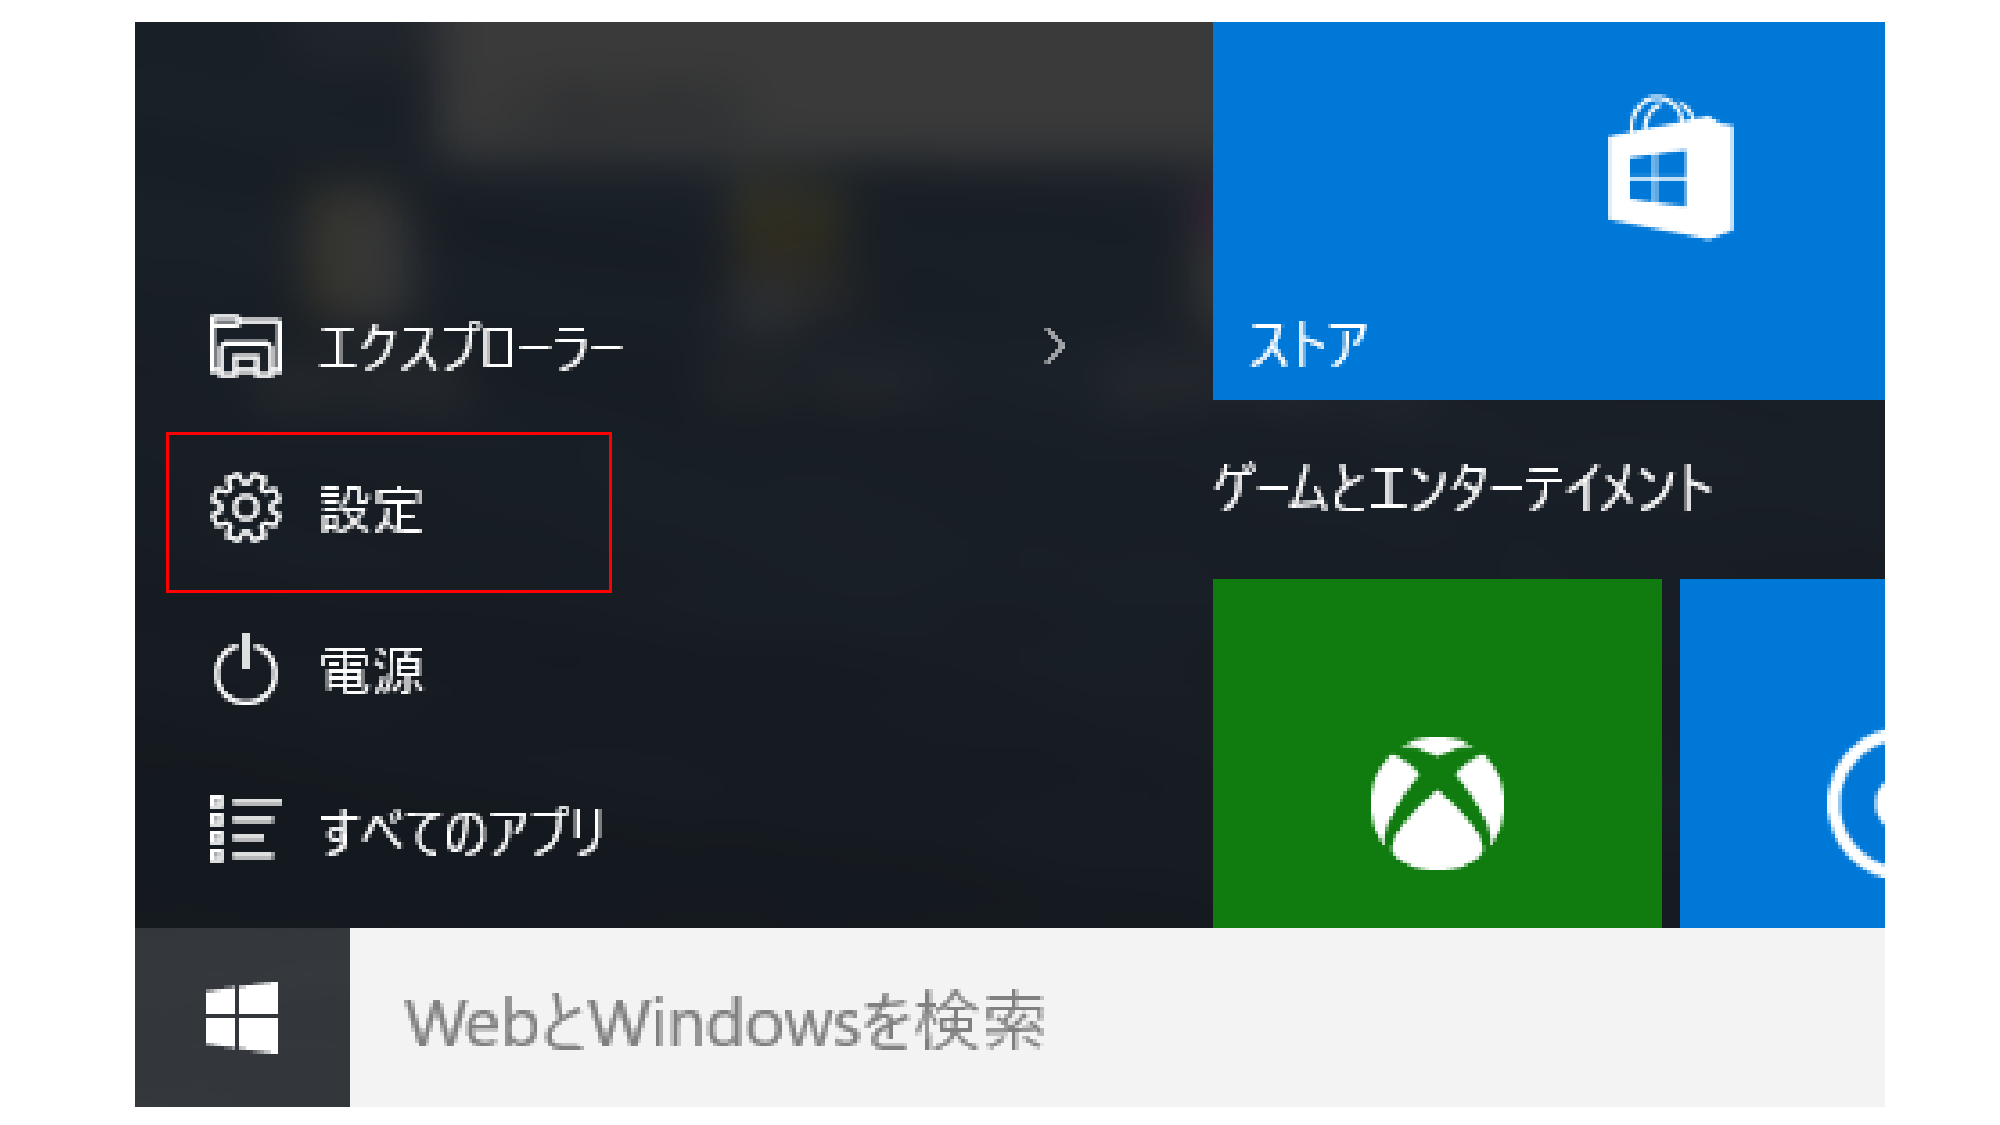
\includegraphics[width=12cm]{win-vpn1.pdf}
 \end{center}
 \caption{VPNの設定1}
 \label{winvpn1}
\end{figure}

\begin{figure}[htbp]
 \begin{center}
  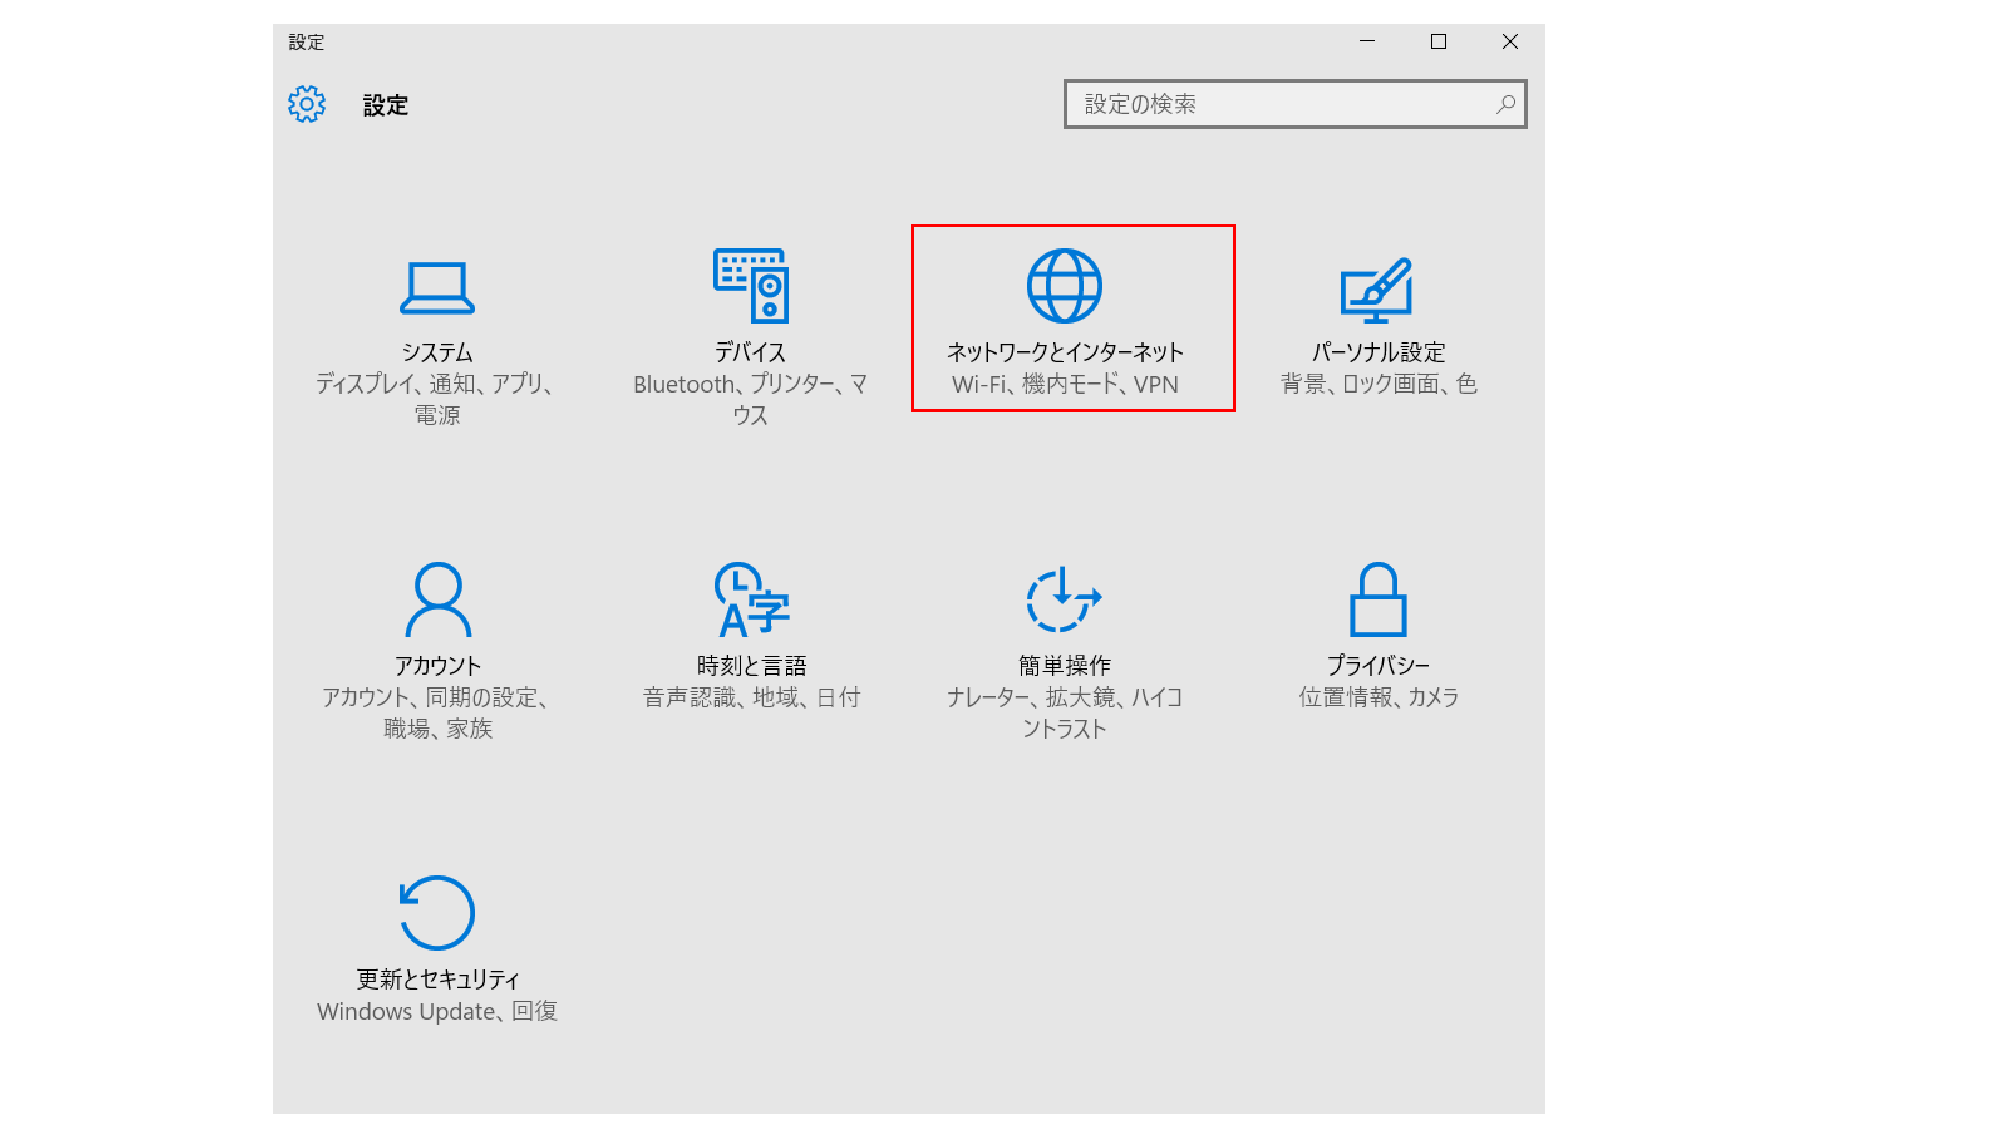
\includegraphics[width=15cm]{win-vpn2.pdf}
 \end{center}
 \caption{VPNの設定2}
 \label{winvpn2}
\end{figure}

\begin{figure}[htbp]
 \begin{center}
  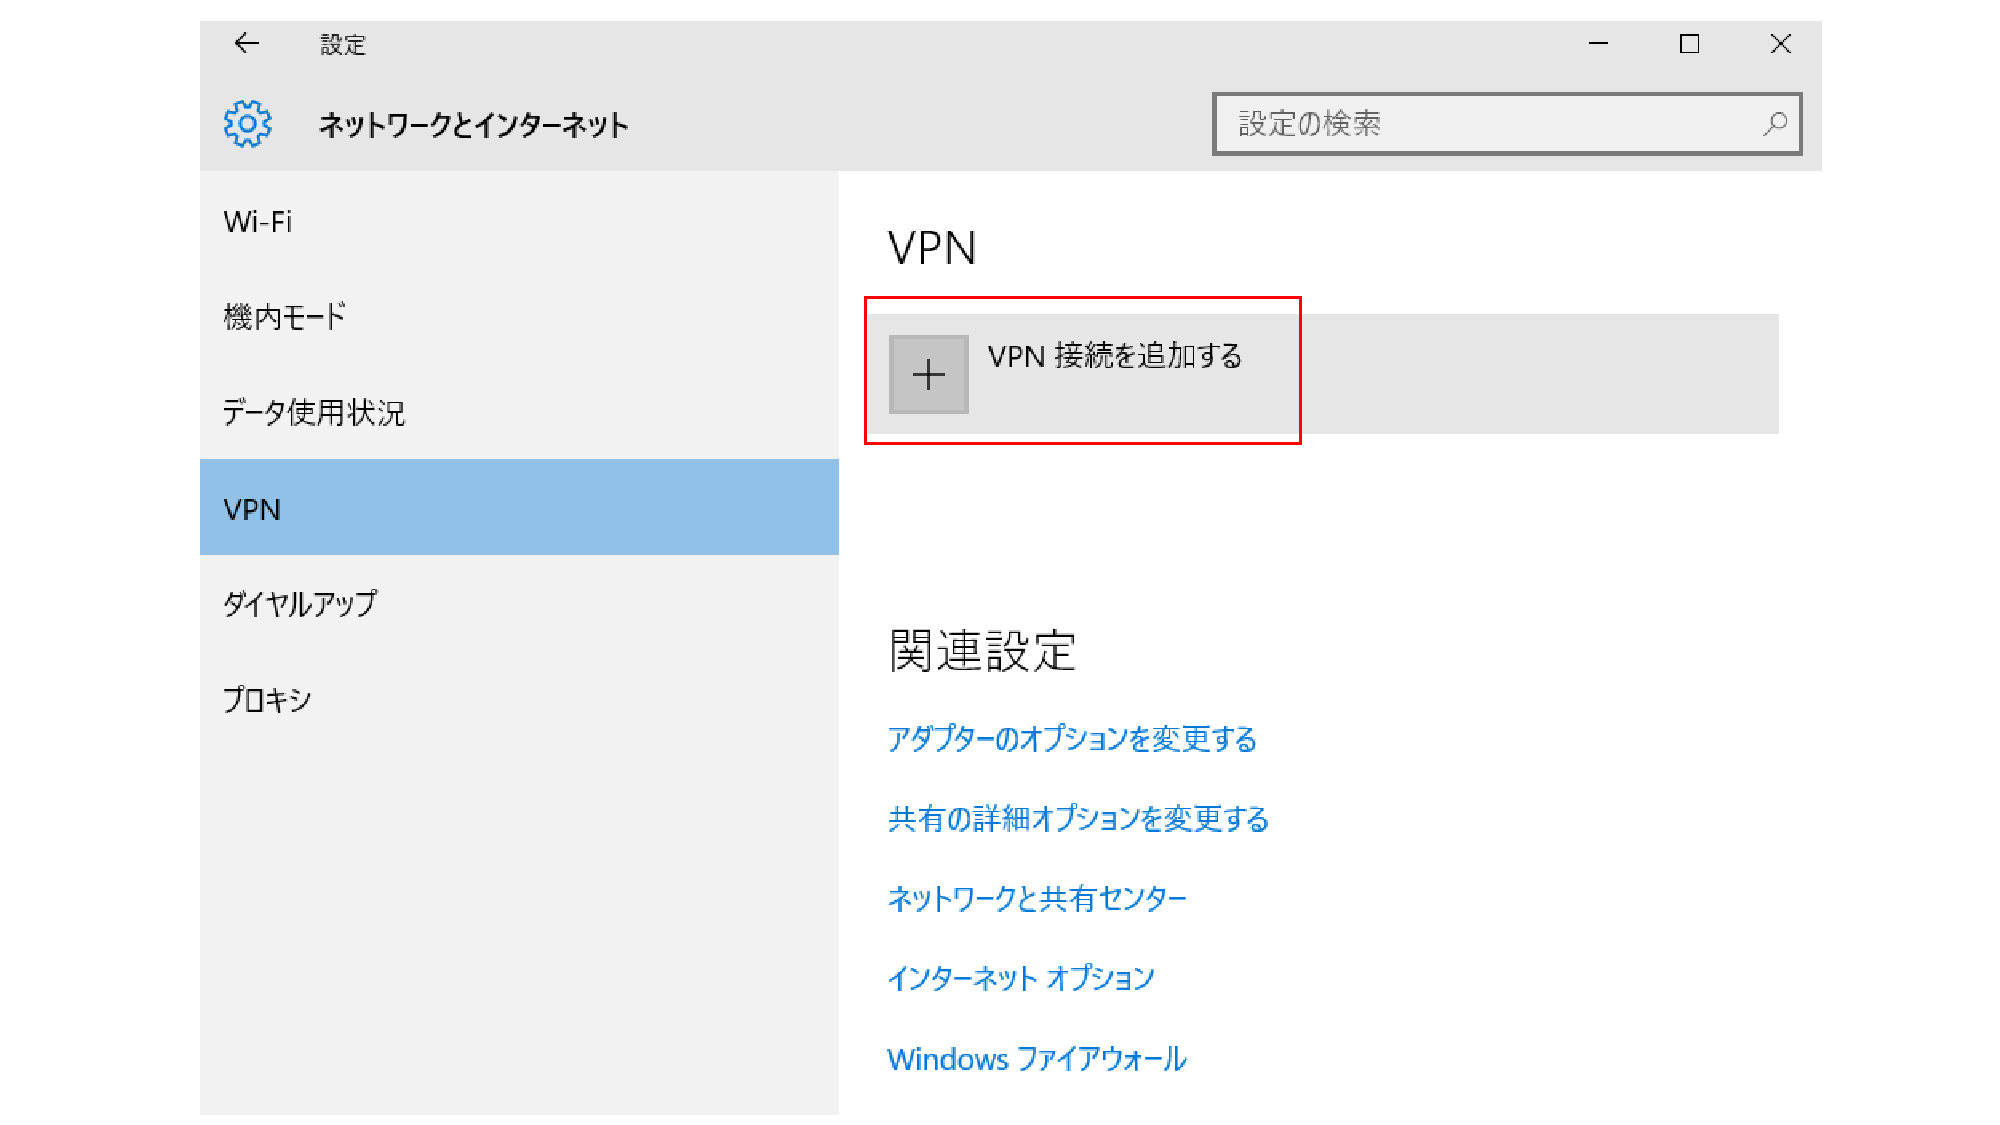
\includegraphics[width=17cm]{win-vpn3.pdf}
 \end{center}
 \caption{VPNの設定3}
 \label{winvpn3}
\end{figure}

\begin{figure}[htbp]
 \begin{center}
  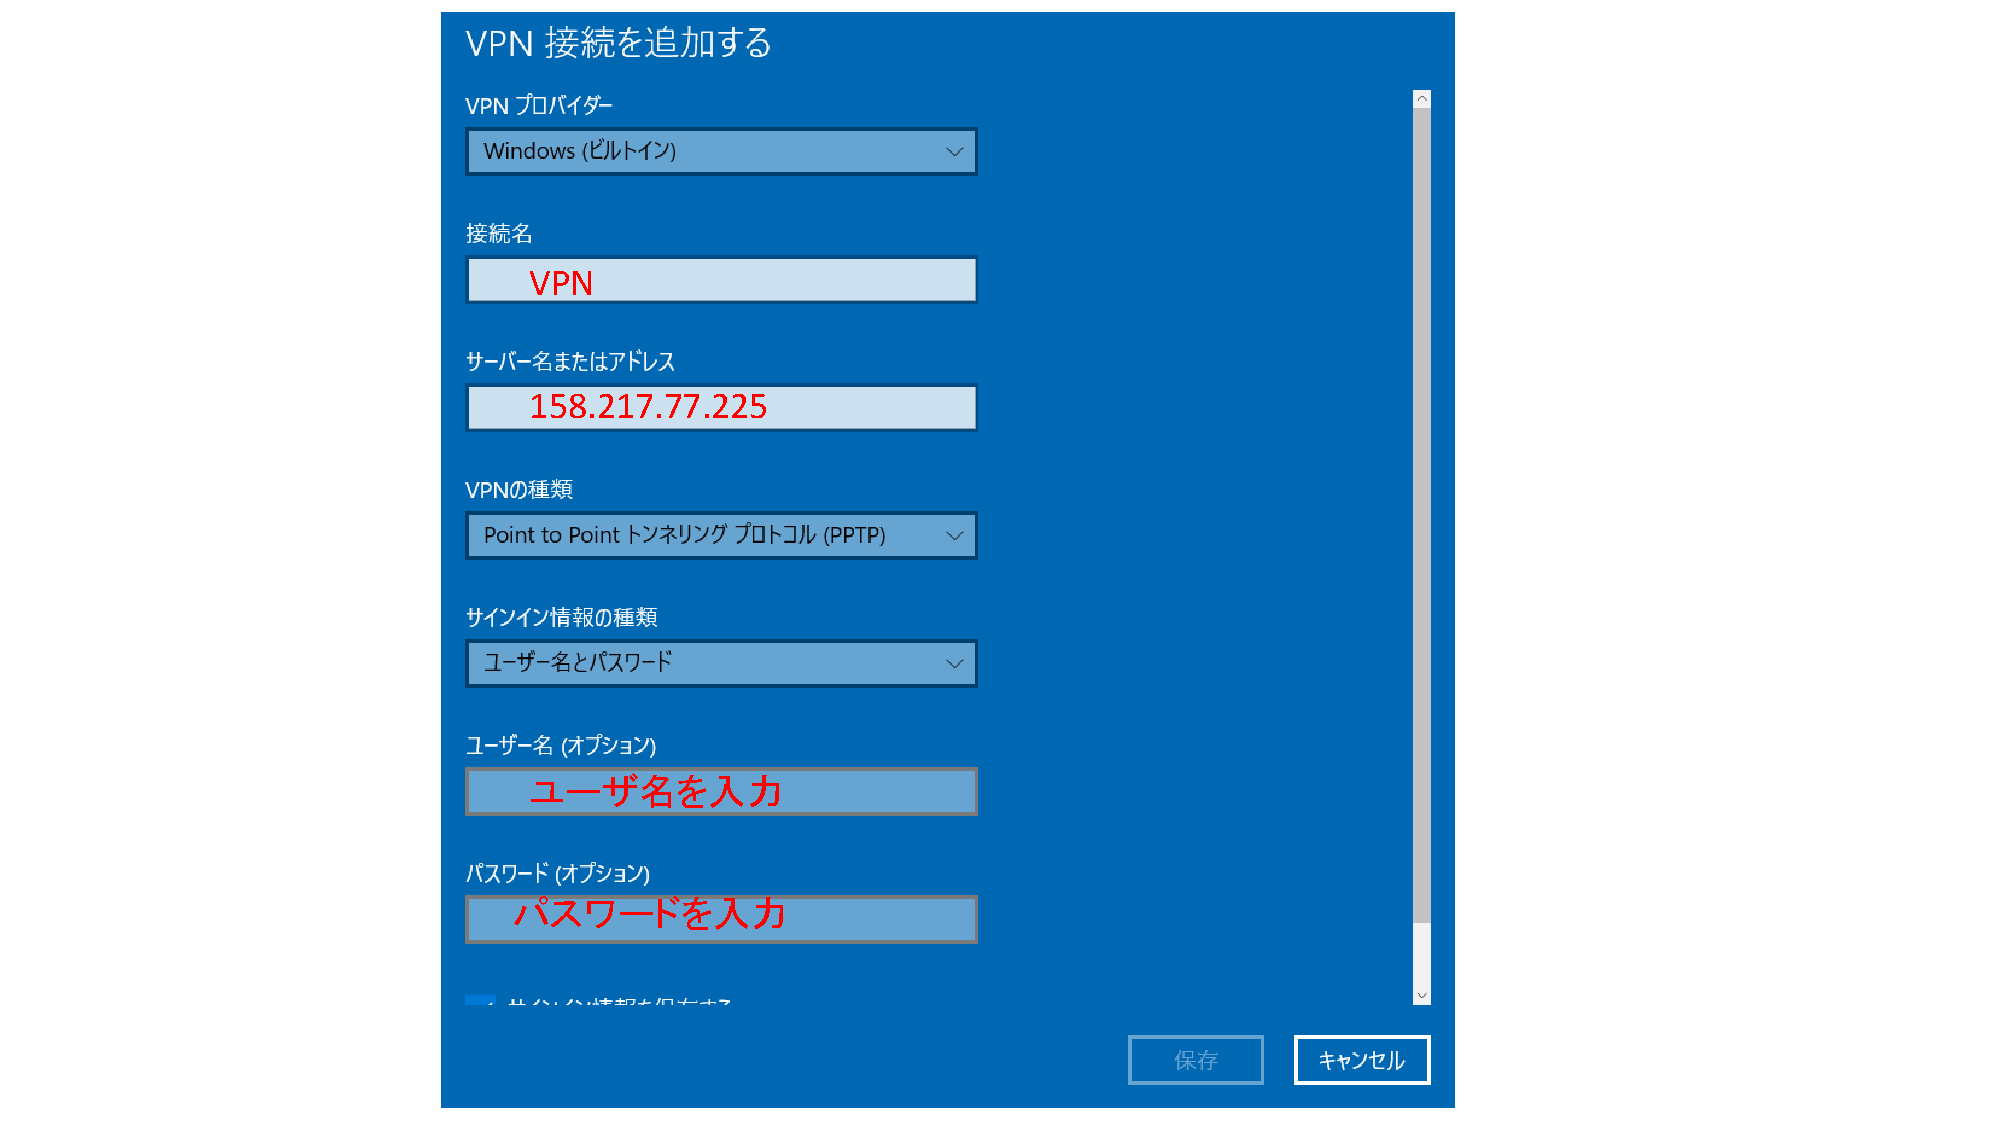
\includegraphics[width=18cm]{win-vpn4.pdf}
 \end{center}
 \caption{VPNの設定4}
 \label{winvpn4}
\end{figure}

\begin{figure}[htbp]
 \begin{center}
  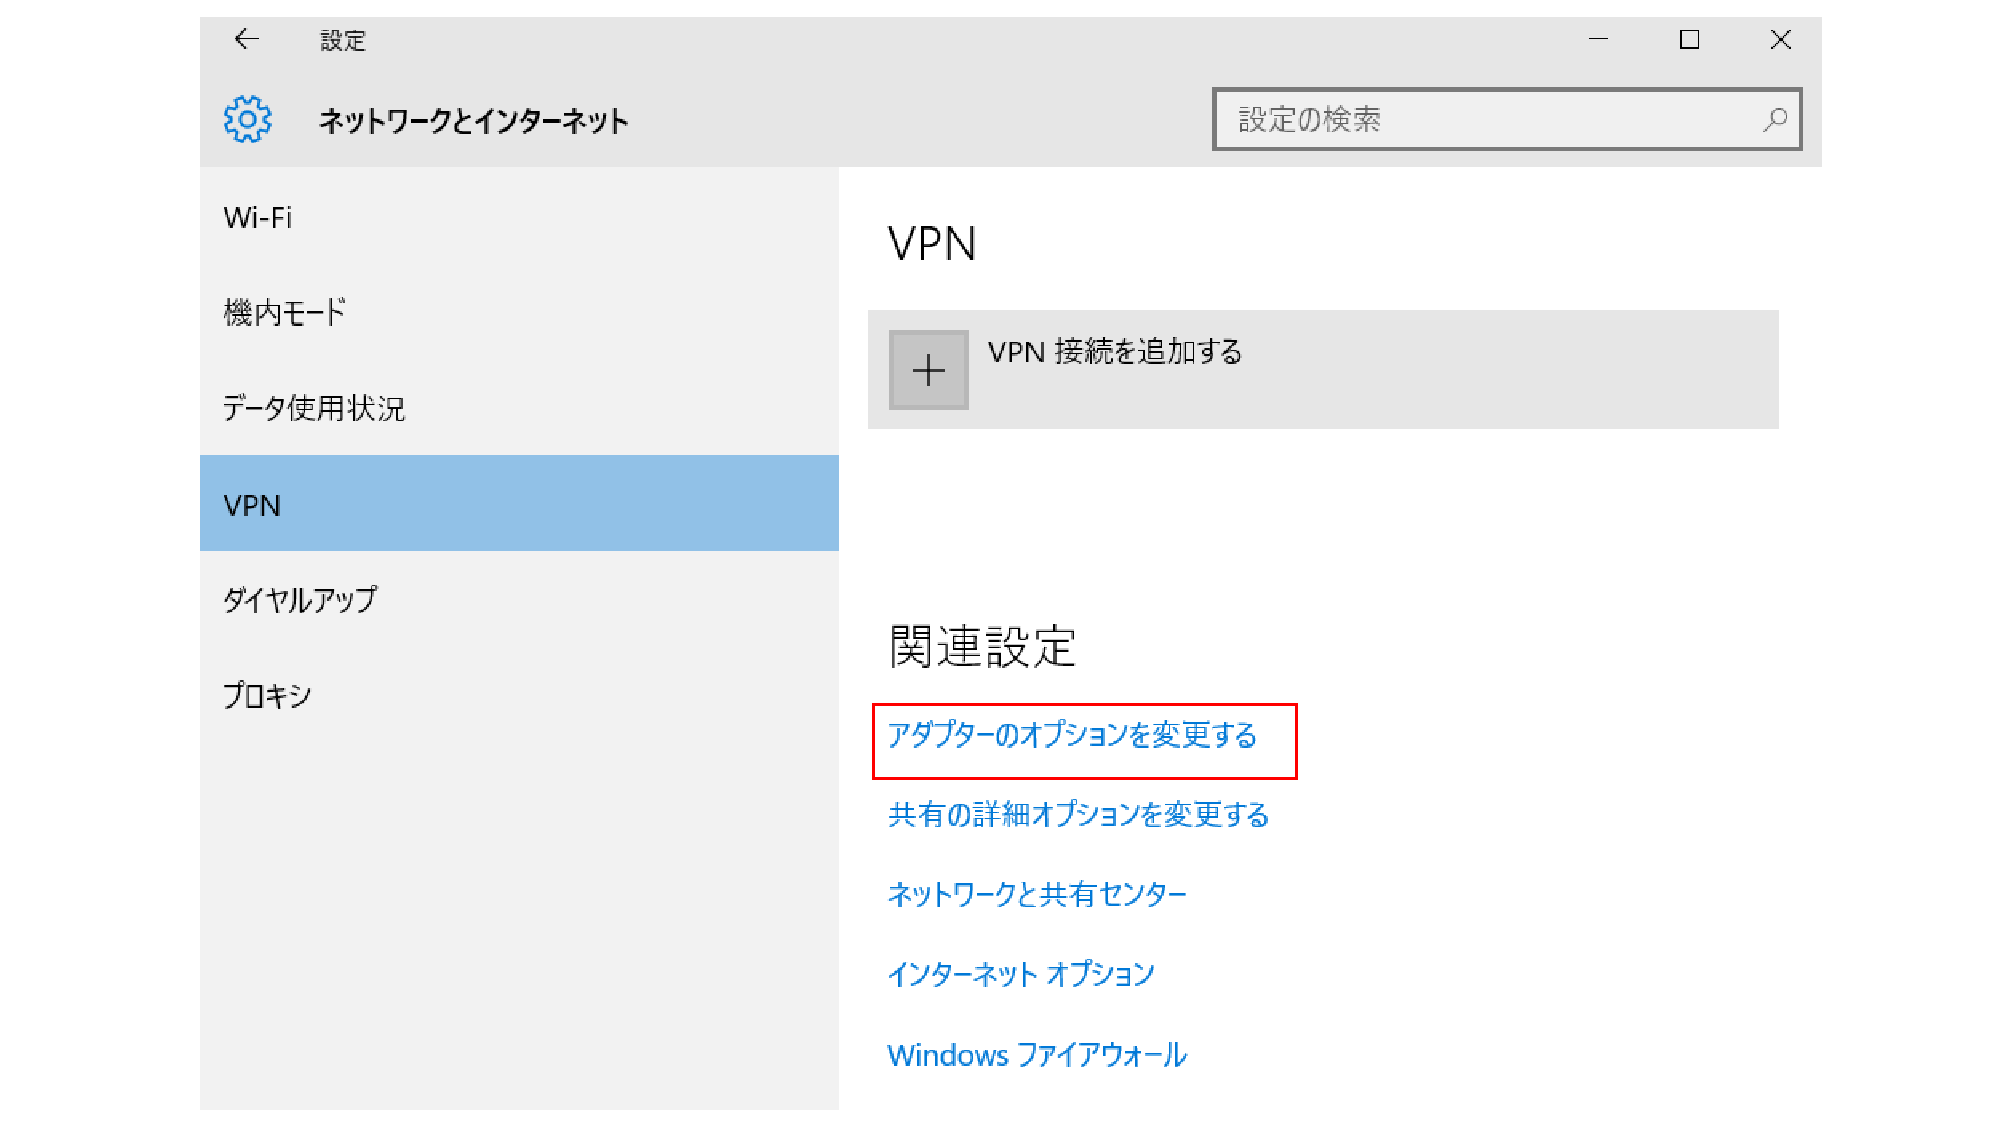
\includegraphics[width=15cm]{win-vpn5.pdf}
 \end{center}
 \caption{VPNの設定5}
 \label{winvpn5}
\end{figure}

\begin{figure}[htbp]
 \begin{center}
  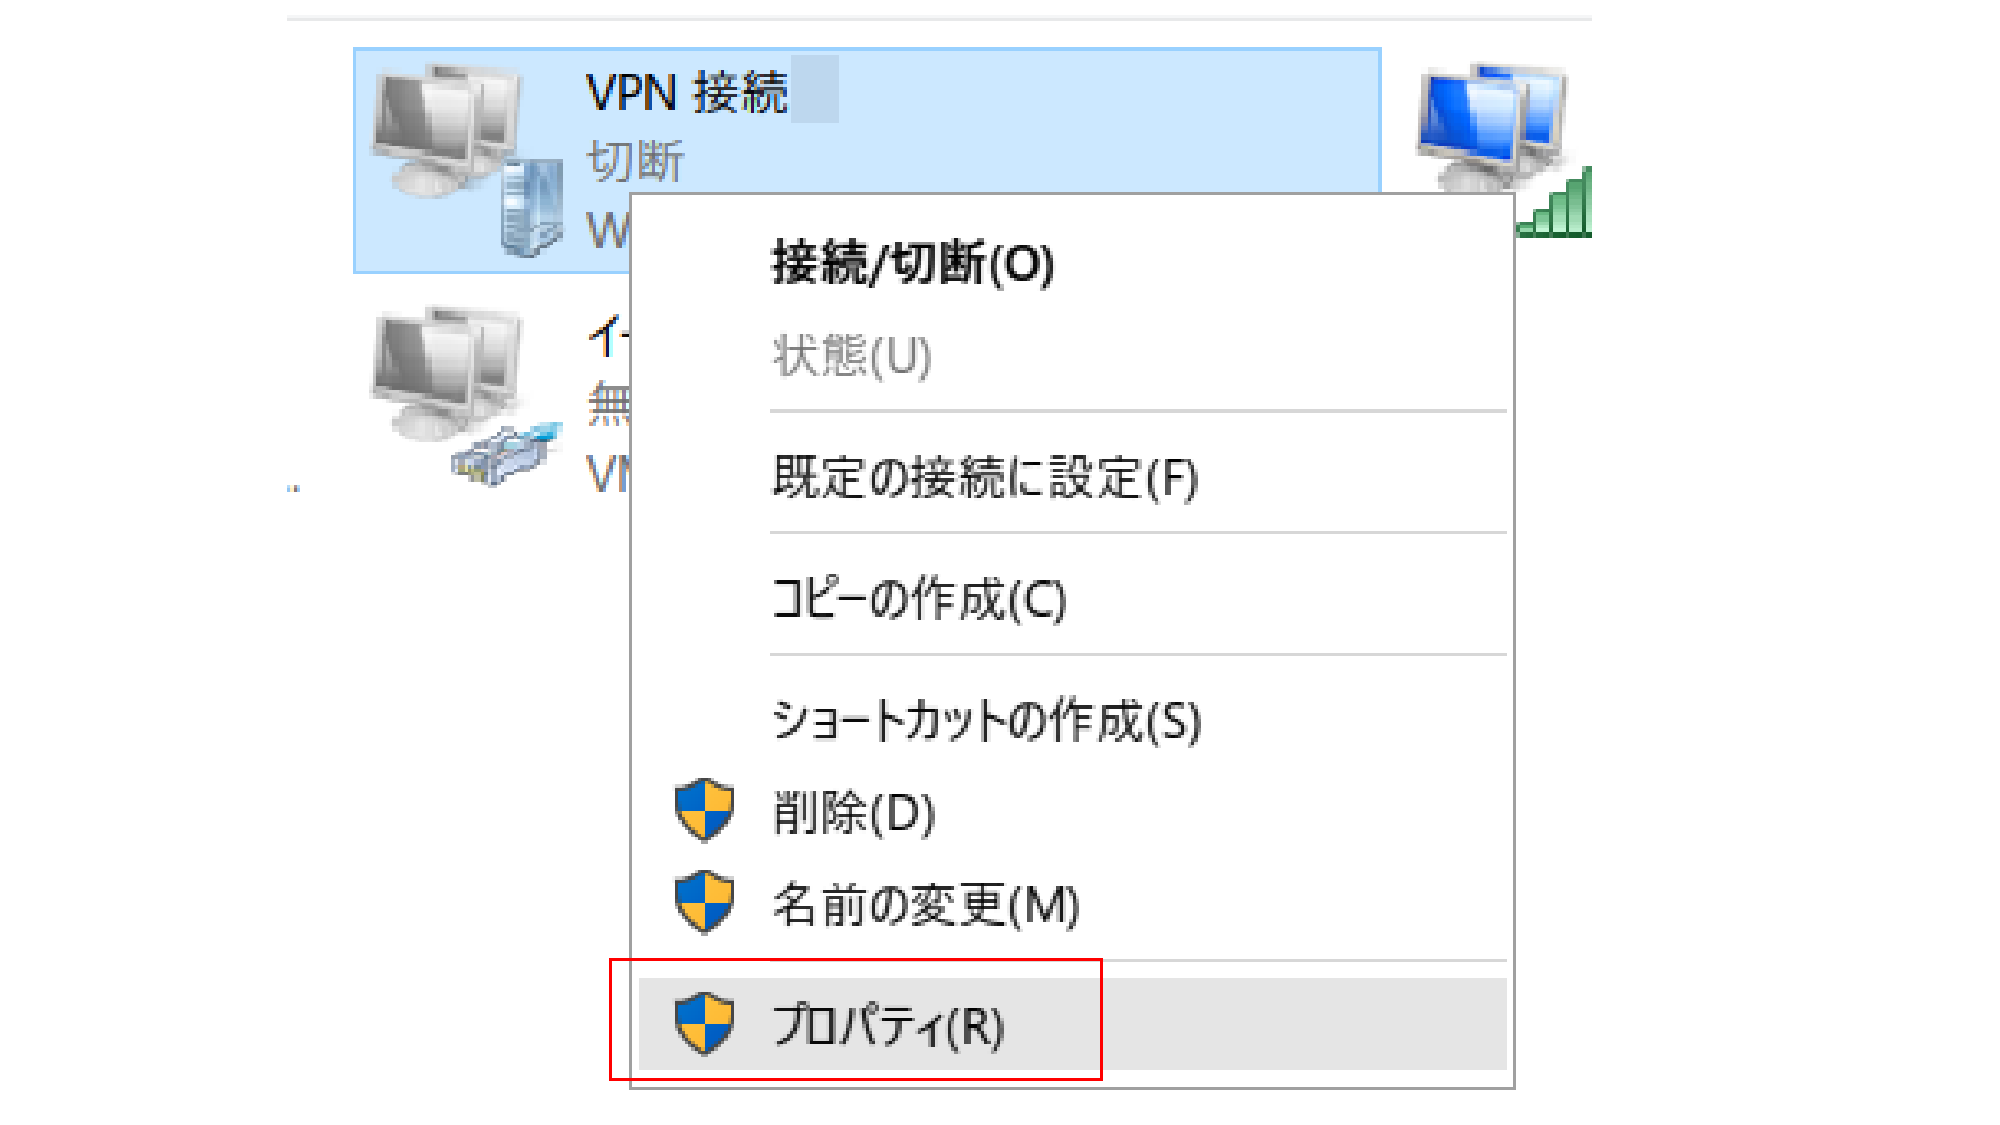
\includegraphics[width=17cm]{win-vpn6.pdf}
 \end{center}
 \caption{VPNの設定6}
 \label{winvpn6}
\end{figure}

\begin{figure}[htbp]
 \begin{center}
  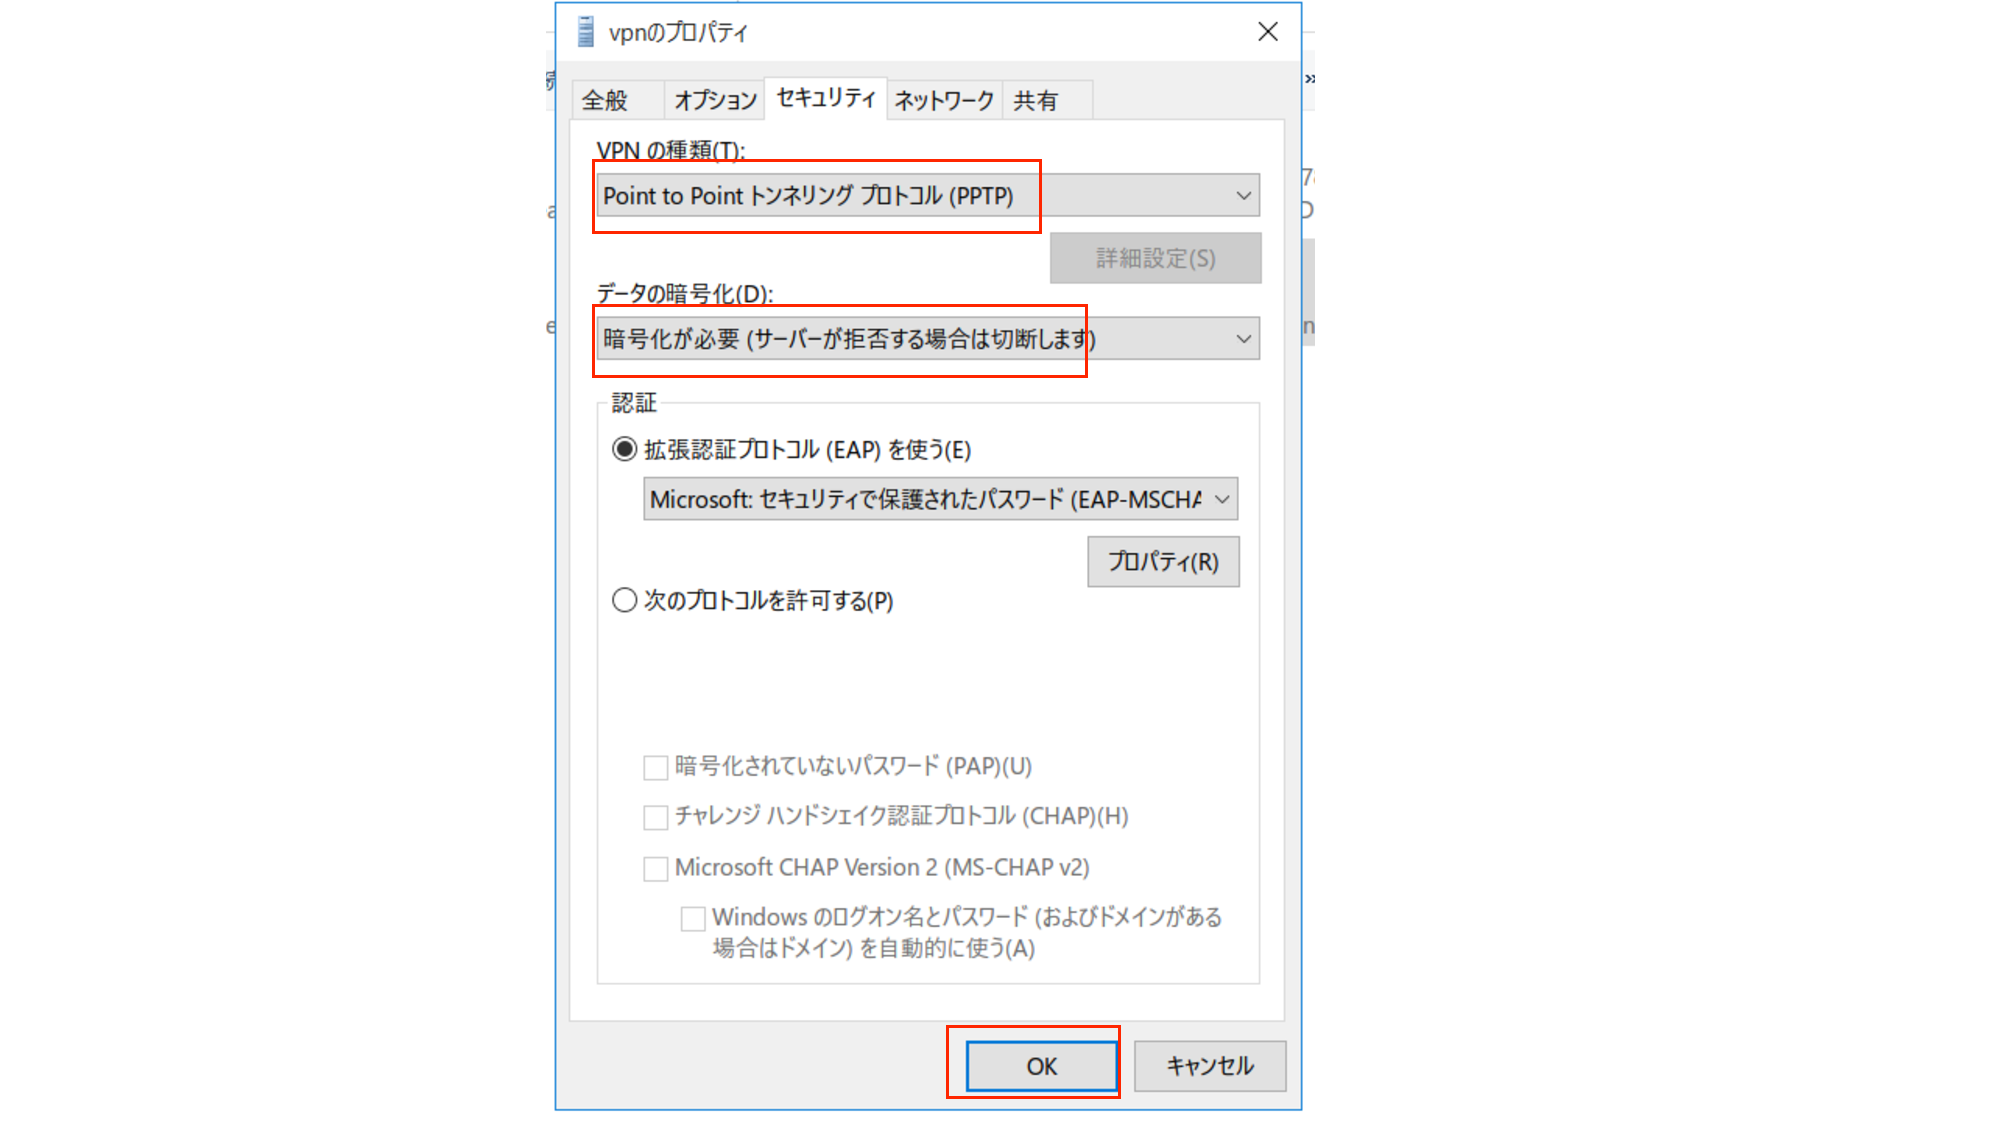
\includegraphics[width=19cm]{win-vpn7.pdf}
 \end{center}
 \caption{VPNの設定7}
 \label{winvpn7}
\end{figure}

\begin{figure}[htbp]
 \begin{center}
  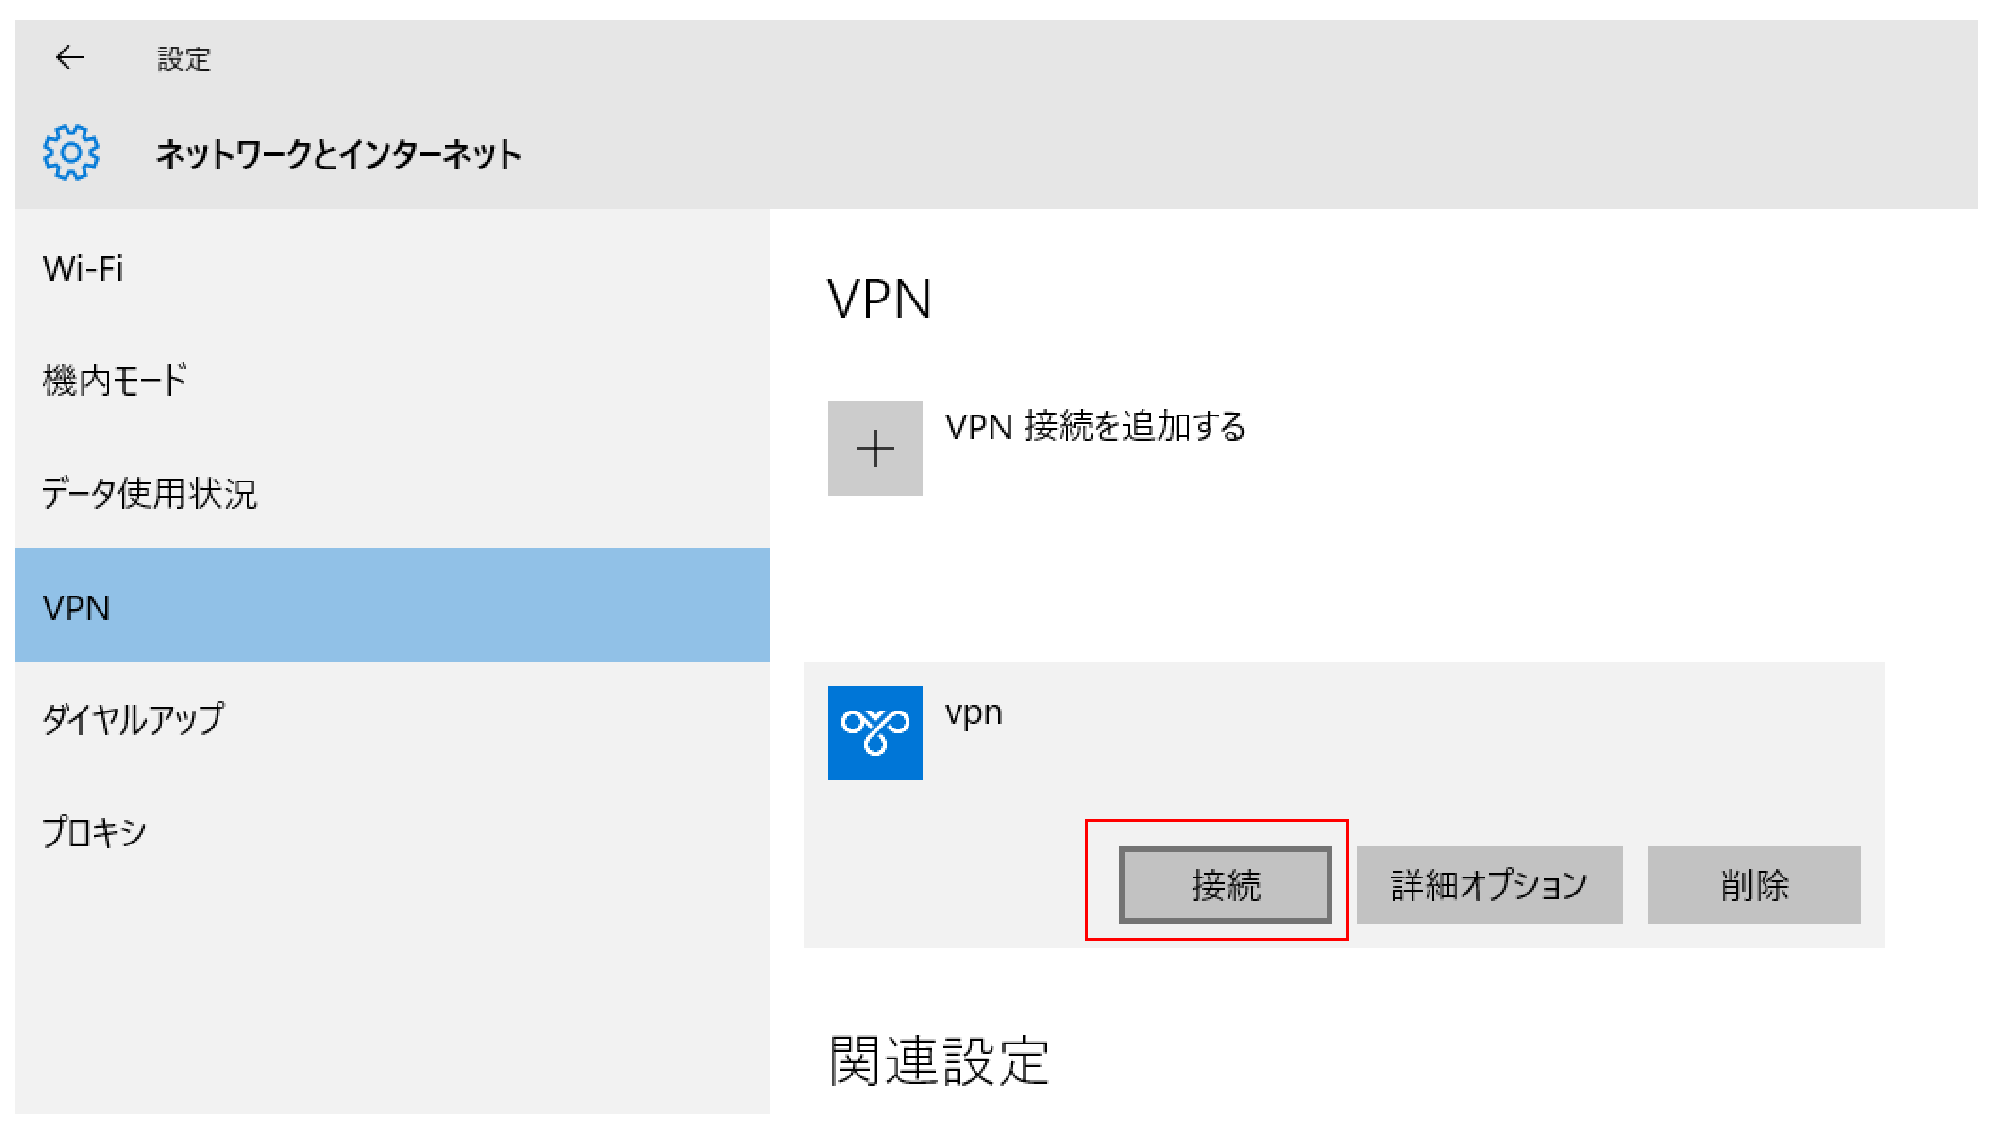
\includegraphics[width=15cm]{win-vpn8.pdf}
 \end{center}
 \caption{VPNの設定8}
 \label{winvpn8}
\end{figure}

%\include{vpn}
\section{TCP/UDP}
TCP/IP階層モデルにおけるトランスポート層は,ネットワーク層で端末(ノード)間の橋渡しがなされ送られてきたパケットについて,これが届いたかどうかの確認をしたり,これの順序を整理したり,データが壊れていないかを確認したり,大きすぎるデータを分割したり,データの送信量を制御する.また,データを適切なアプリケーションに引き渡す役割もある.

トランスポート層の代表的なプロトコルとして,TCPとUDPがある.これら二つの違いをごく簡単に説明すると,信頼性のある通信を重視するものがTCP,伝送効率の高い通信を重視するものがUDPである,となる.

それではまず,UDPについて説明を始めよう.

\subsection{UDP}
UDPは,通信の信頼性よりも,速さやリアルタイム性が要求されるような場合において使用されるプロトコルである.UDPのヘッダを図\ref{tcpudp-udp-header}に示す.

\begin{figure}[htb]
  \centering
  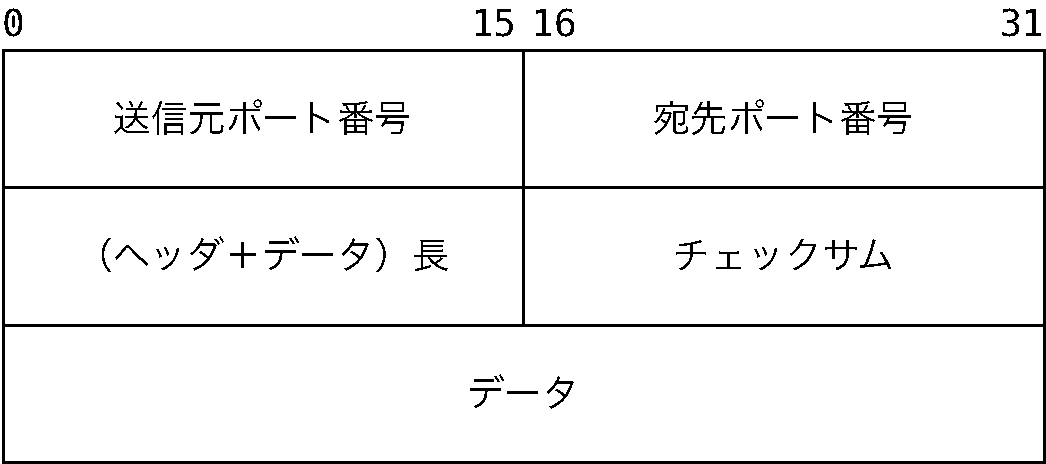
\includegraphics[bb=0 0 502 222, width=10cm]{tcpudp-udp-header.pdf}
  \caption{UDPヘッダ}
  \label{tcpudp-udp-header}
\end{figure}

UDPのヘッダは,このように極めてシンプルな構造になっている.データを転送する際,送信側はチェックサムの計算を行って送信するだけであり,受信側はチェックサムを計算してデータに誤りが無いか確認した後,受け取った順にそのままアプリケーションに渡すだけである.後述するTCPにおいて使われている3-way handshakeや確認応答,順序制御,再送制御,伝送制御などの機能は無く,処理がシンプルであるが故に高速なのである.

ただし,パケットが確実に到達するという保証が無いため,何らかの原因でパケットロスが発生した場合にでも処理を継続できるようにアプリケーション側で工夫する必要がある.

このプロトコルは,DNSやNTP,DHCPなどのデータ量の少ないものや,音楽や映画などのストリーミング配信,またオンラインゲームのようなリアルタイム性が要求されるもので使われることが多い.

\subsection{TCP}
TCPは,信頼性の高い通信を実現するために使用されるプロトコルである.TCPのヘッダを図\ref{tcpudp-tcp-header}に示す.シーケンス番号では送信するデータの通し番号を管理しており,確認応答番号(ACK番号)ではどのシーケンス番号までデータを受信したかを示している.

\begin{figure}[htb]
  \centering
  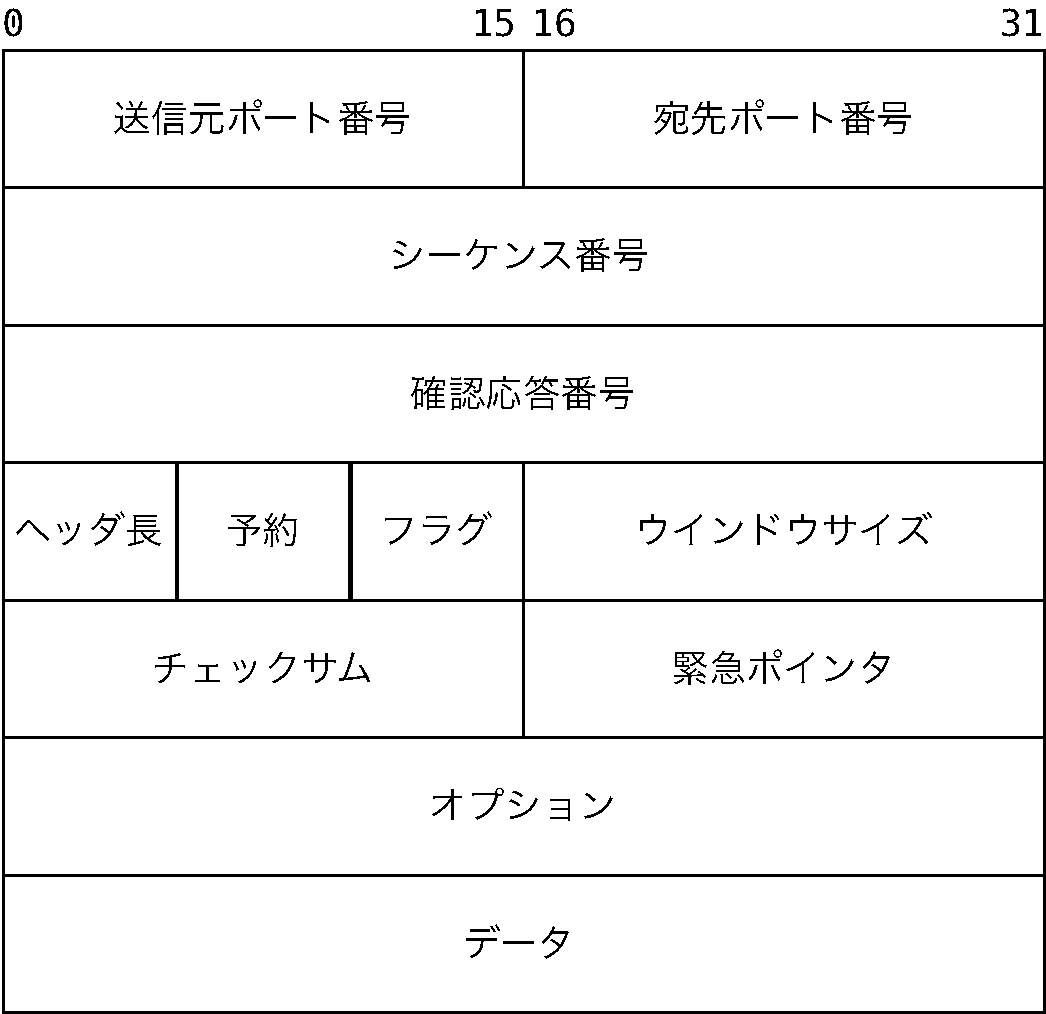
\includegraphics[bb=0 0 502 486, width=10cm]{tcpudp-tcp-header.pdf}
  \caption{TCPヘッダ}
  \label{tcpudp-tcp-header}
\end{figure}

フラグでは,そのTCPパケットがどのような種類のものなのかを示している.フラグ名とその意味を整理したものを表\ref{tcpudp-tcp-flaglist}に示す.

\begin{table}[htb]
  \centering
  \caption{TCPのフラグ一覧}
  \label{tcpudp-tcp-flaglist}
  \begin{tabular}{|c|l|} \hline
    URG & このTCPパケット内に緊急データが含まれていることを示す \\ \hline
    ACK & TCPヘッダ内に有効なACK番号が含まれていることを示す \\ \hline
    PSH & 受信したデータをすぐにアプリケーションに引き渡すよう要求する \\ \hline
    RST & TCP接続の中断,拒否を示す \\ \hline
    SYN & 3-way handshake時に使われ,ACK番号を同期させる \\ \hline
    FIN & TCP接続を終了させる \\ \hline
  \end{tabular}
\end{table}

また,TCPをベースとするHTTP通信の例を表\ref{tcpudp-http-sample}に示す.これを参考にしつつTCP通信の特徴を説明していく.

\begin{table}[htb]
  \centering
  \caption{HTTP通信の例}
  \label{tcpudp-http-sample}
  \begin{tabular}{|c|c|c|l|l|l|l|} \hline
      Src & Dst & Flag & Length & Seq num & Ack num & HTTP \\ \hline \hline
      Client & Server & SYN & 0 & 0 & 0 & \\ \hline
      Server & Client & SYN,ACK & 0 & 0 & 1 & \\ \hline
      Client & Server & ACK & 0 & 1 & 1 & \\ \hline
      Client & Server & PSH,ACK & 394 & 1 & 1 & \shortstack{GET /$\sim$bob/sample.html \\ HTTP/1.1} \\ \hline
      Server & Client & PSH, ACK & 353 & 1 & 395 & HTTP/1.1 200 OK \\ \hline
      Client & Server & ACK & 0 & 395 & 354 & \\ \hline
      Server & Client & FIN,ACK & 0 & 354 & 395 & \\ \hline
      Client & Server & ACK & 0 & 395 & 355 & \\ \hline
  \end{tabular}
\end{table}

まず,TCPではUDPのようにデータを一方的に送りつけるのではなく,事前に接続を確立する手順を踏む.この手順のことを3-way handshakeと呼ぶ.表\ref{tcpudp-http-sample}の例では上から三つ分のパケットがこれにあたる.

まず,接続する側(クライアント)は接続される側(サーバ)に対してSYNフラグを立てたパケットを送信し,上りのコネクション確立を試みる.これを受け取ったサーバ側はACKとSYNフラグを立てたパケットを送信し,上りのコネクション確立を承認するとともに,下りのコネクション確立を試みる.これを受け取ったクライアント側はACKフラグを立てたパケットをサーバに送信し,下りのコネクション確立を承認する.以上の手順により信頼性のあるコネクション確立が完了し,これ以降でデータの通信が行われる.

送信したデータが全て受信側に到着したかを確認するために,データのバイト数とシーケンス番号,ACK番号が用いられる.例として送信側が394バイトのデータを送信するケースを考えてみる.送信側はデータと共にシーケンス番号を送信する.これを受け取った側はデータのバイト数とシーケンス番号を足し,これをACK番号として送信側に送る.これを受け取った送信側で,受け取ったACK番号が,送信したデータのバイト数と送信時のシーケンス番号を足したものと一致していれば全てのデータが到達していることがわかる.もしここで数値が一致しなければ,再度データを送信することになる.

\subsubsection{パケット転送効率の改善}
上述の通り,TCPではパケットを送信し,ACKを受け取るという流れを繰り返してデータ転送を行う.だがこのままだとパケット送信からACK受信までの時間(RTT,Round Trip Time)の関係で,送信側で送信準備ができていたとしてもACKを受け取れない限り送信できず,転送の効率が悪化する.

これを改善するために,TCPではウインドウ制御の一つの方法である,スライディングウインドウ方式という仕組みがある.TCPヘッダの中にはウインドウサイズという,受信側が受信できるデータ量を送信側に知らせるフィールドがある.送信側はこのウインドウサイズをもとに,ACKを待たずに次々にパケットを送信する.一定量パケットを送信したらACKパケットを待ち,ACKパケットを受け取ったらまた次のパケットを送っていくという方法になる.ウインドウサイズに収まるサイズのデータを送り,どこか一つのパケットに対応するACKを受信したらそこまでのパケットは到達しているとみなしてウインドウを横にずらして新たなパケットを送信するイメージである.

スライディングウインドウ方式により,送信側の転送効率は上がる.だがこれではネットワークの混雑度合いを考慮できておらず,次々にパケットを送信し続けてしまうことで混雑度合いをさらに悪化させてしまう.この問題に対処するために,輻輳制御という方法が用いられている.初めからウインドウサイズ一杯でパケットを送信するのではなく,徐々に転送量を増やしていき,輻輳が発生した場合に再度ウインドウサイズを小さくして再度転送量を増やすというものだ.

以上の仕組みはパケットの送信側において,効率よくパケットを送信するための仕組みである.ただ,パケットの受信側で処理に時間がかかるような場合,次々にパケットを送信されてしまうと受信側は処理がパンクしてしまう恐れがある.これを回避するためにもウインドウサイズは用いられる.パケットが送られてくるたびにウインドウサイズを減らして送信側に通知し,処理がパンクしそうになるとウインドウサイズをゼロにして送信側に通知する.これにより送信側は受信側の状況を見てパケットの送信を中断でき,受信側で余裕ができたらこれを通知して通信を再開させたり(ウインドウ更新通知),送信側が受信側に余裕ができたかを問い合わせて通信を再開することができる(ウインドウプローブ).

以上のような仕組みを用いてTCPは転送効率の向上を行っている.

\subsection{チェックサム}
TCPやUDP(とIP)にはチェックサムという仕組みがあり,これを用いてデータの損傷を検出できるようになっている.計算に用いるのは,TCPあるいはUDPヘッダとデータ,擬似ヘッダの三つである.擬似ヘッダとは仮想的なヘッダで,実際のTCPパケット内には含まれておらず,チェックサムを計算する際にのみ利用する.

送信側は,まずTCPあるいはUDPヘッダとデータ,擬似ヘッダの三つで合わせて16ビットの整数倍になるようにデータの長さを調節する.また,あらかじめチェックサムフィールドをゼロで埋めておく.そして先ほど調節したデータとTCPあるいはUDPヘッダ,擬似ヘッダについて16ビットごとに1の補数を求め(ビット反転させ),その総和を求め,これの1の補数をチェックサムフィールドに入れて送信する.
受信側は,同様に擬似ヘッダを付けた状態で16ビットずつ1の補数を求め,その総和を計算する.データが破損していない場合はこの計算結果が0xFFFFになる.これは送信側がチェックサムフィールドに入れた値がチェックサムフィールド以外の補数和の1の補数であり,受信側が行っていることはチェックサムフィールド以外の補数和にその1の補数を足す処理をしている,ということから分かるのではないかと思う.

\subsection{ポート番号}
TCP/IP階層モデルにおけるトランスポート層ではアプリケーション層との間でのデータのやり取りを担うが,どのアプリケーションからのデータなのか,また,どのアプリケーションに対してのデータなのかを識別するためにポート番号が用いられる.ポート番号はTCPとUDPでそれぞれ0番から65535番まであり,その中で大きく三つの種類に分けられる.この分け方を表\ref{tcpudp-kind-of-port}に示す.
\begin{table}[htb]
    \centering
    \caption{ポート番号の種類}
    \label{tcpudp-kind-of-port}
    \begin{tabular}{|c|c|} \hline
        Well Known Ports & 0 $\sim$ 1023 \\ \hline
        Registered Ports & 1024 $\sim$ 49151 \\ \hline
        Dynamic and/or Private Ports & 49152 $\sim$ 65535 \\ \hline
    \end{tabular}
\end{table}

まず,0番から1023番まではWell Known Ports(System Ports)と呼ばれ,例えばSSH(22)やHTTP(80),HTTPS(443)などの一般的によく利用される主要なサービスのために登録されている.また,Unix系OSにおいてこの範囲のポートは管理者の権限を持つユーザのみが利用できる.1024番から49151番まではRegistered Ports(User Ports)と呼ばれ,一般的なサービスではないが,登録制によって割り当てられるものとなる.49152番から65535番まではDynamic and/or Private Portsと呼ばれ,クライアント側で自動的に利用されるもの,あるいはユーザが自由に利用できるもの,とされている.
これらポート番号の管理や割り当ては,IANA(Internet Assigned Numbers Authority)が行っている.


\section{アプリケーション層}
アプリケーション層は,OSI参照モデルの第7層,またTCP/IP参照モデルでは第4層に位置するレイヤのことを指す.
このレイヤは,ネットワークを介したアプリケーション(ソフトウェア,プログラム)の通信プロトコルを定義している.
これらのアプリケーションに対して,透過的なネットワーク通信を実現するインタフェースを提供し,
ユーザアプリケーションによる情報のやり取りを容易にしている.
例えば,インターネット上においてデータ通信の要となっているのはHTTPとよばれるプロトコルである.
従って,普段Webブラウザでインターネット上のページを見るときは,そのページを提供しているWebサーバとの間で
HTTP通信を行っていることが多い.

アプリケーション層で定義されているプロトコルには,代表的なものとして,HTTPやDHCP,DNS,SMTP,Telnet,FTPが存在する.
この他にも切りがないほど数多くのプロトコルが定義されているが,
本節では,そのなかでも特にメジャーなプロトコルについて説明する.

\subsection{HTTP}
HTTP(HyperText Transfer Protocol)とは,インターネット上においてコンテンツ(HTML,テキスト,画像等)を
送信するための規定を定めたものである.
現在の主流なバージョンは,HTTP/1.1とHTTP/2.0である.近年は,HTTP/2.0の仕様が標準として定められたことにより,
続々とHTTP/2サーバが実装されており,今後の主流になると考えられる.
またHTTPでは,デフォルトでTCPの80番ポートを使用する.

HTTPは通信を暗号化しないため,仮に通信を盗聴された場合に内容が閲覧されたり,
通信内容を改ざんされる危険性がある.そのため,HTTPの通信をセキュアにしたHTTPSという規格も存在している.

\subsubsection{HTTP通信の流れ}
HTTPにおける典型的な通信の流れは,まずWebクライアント(通常はWebブラウザ)がWebサーバに存在するコンテンツに対して
HTTPリクエストを発行するところから始まる.
このとき,Webサーバ上にあるコンテンツは,URI(Uniform Resource Identifier)によって一意に識別される.
Webサーバ側はHTTPリクエストを受け取った後,それに対応するHTTPレスポンスをWebクライアントに返す.
HTTP通信は,実際にこのように単純な仕組みで成り立っている.実際の通信の流れを,図\ref{fig:httpflow}に示す.

この例では,Webブラウザを用いて\url{http://www.kansai-u.ac.jp/index.html}というURLにアクセスしようとしている.
Webブラウザは,\url{www.kansai-u.ac.jp}のWebサーバに対して,index.htmlというコンテンツを要求する
HTTPリクエストを送信する.そして,Webサーバ側はindex.htmlを含むHTTPレスポンスを返す.
最後にクライアント側では,レスポンス内容であるindex.htmlをWebブラウザ上に表示している.

\begin{figure}[htbp]
    \centering
    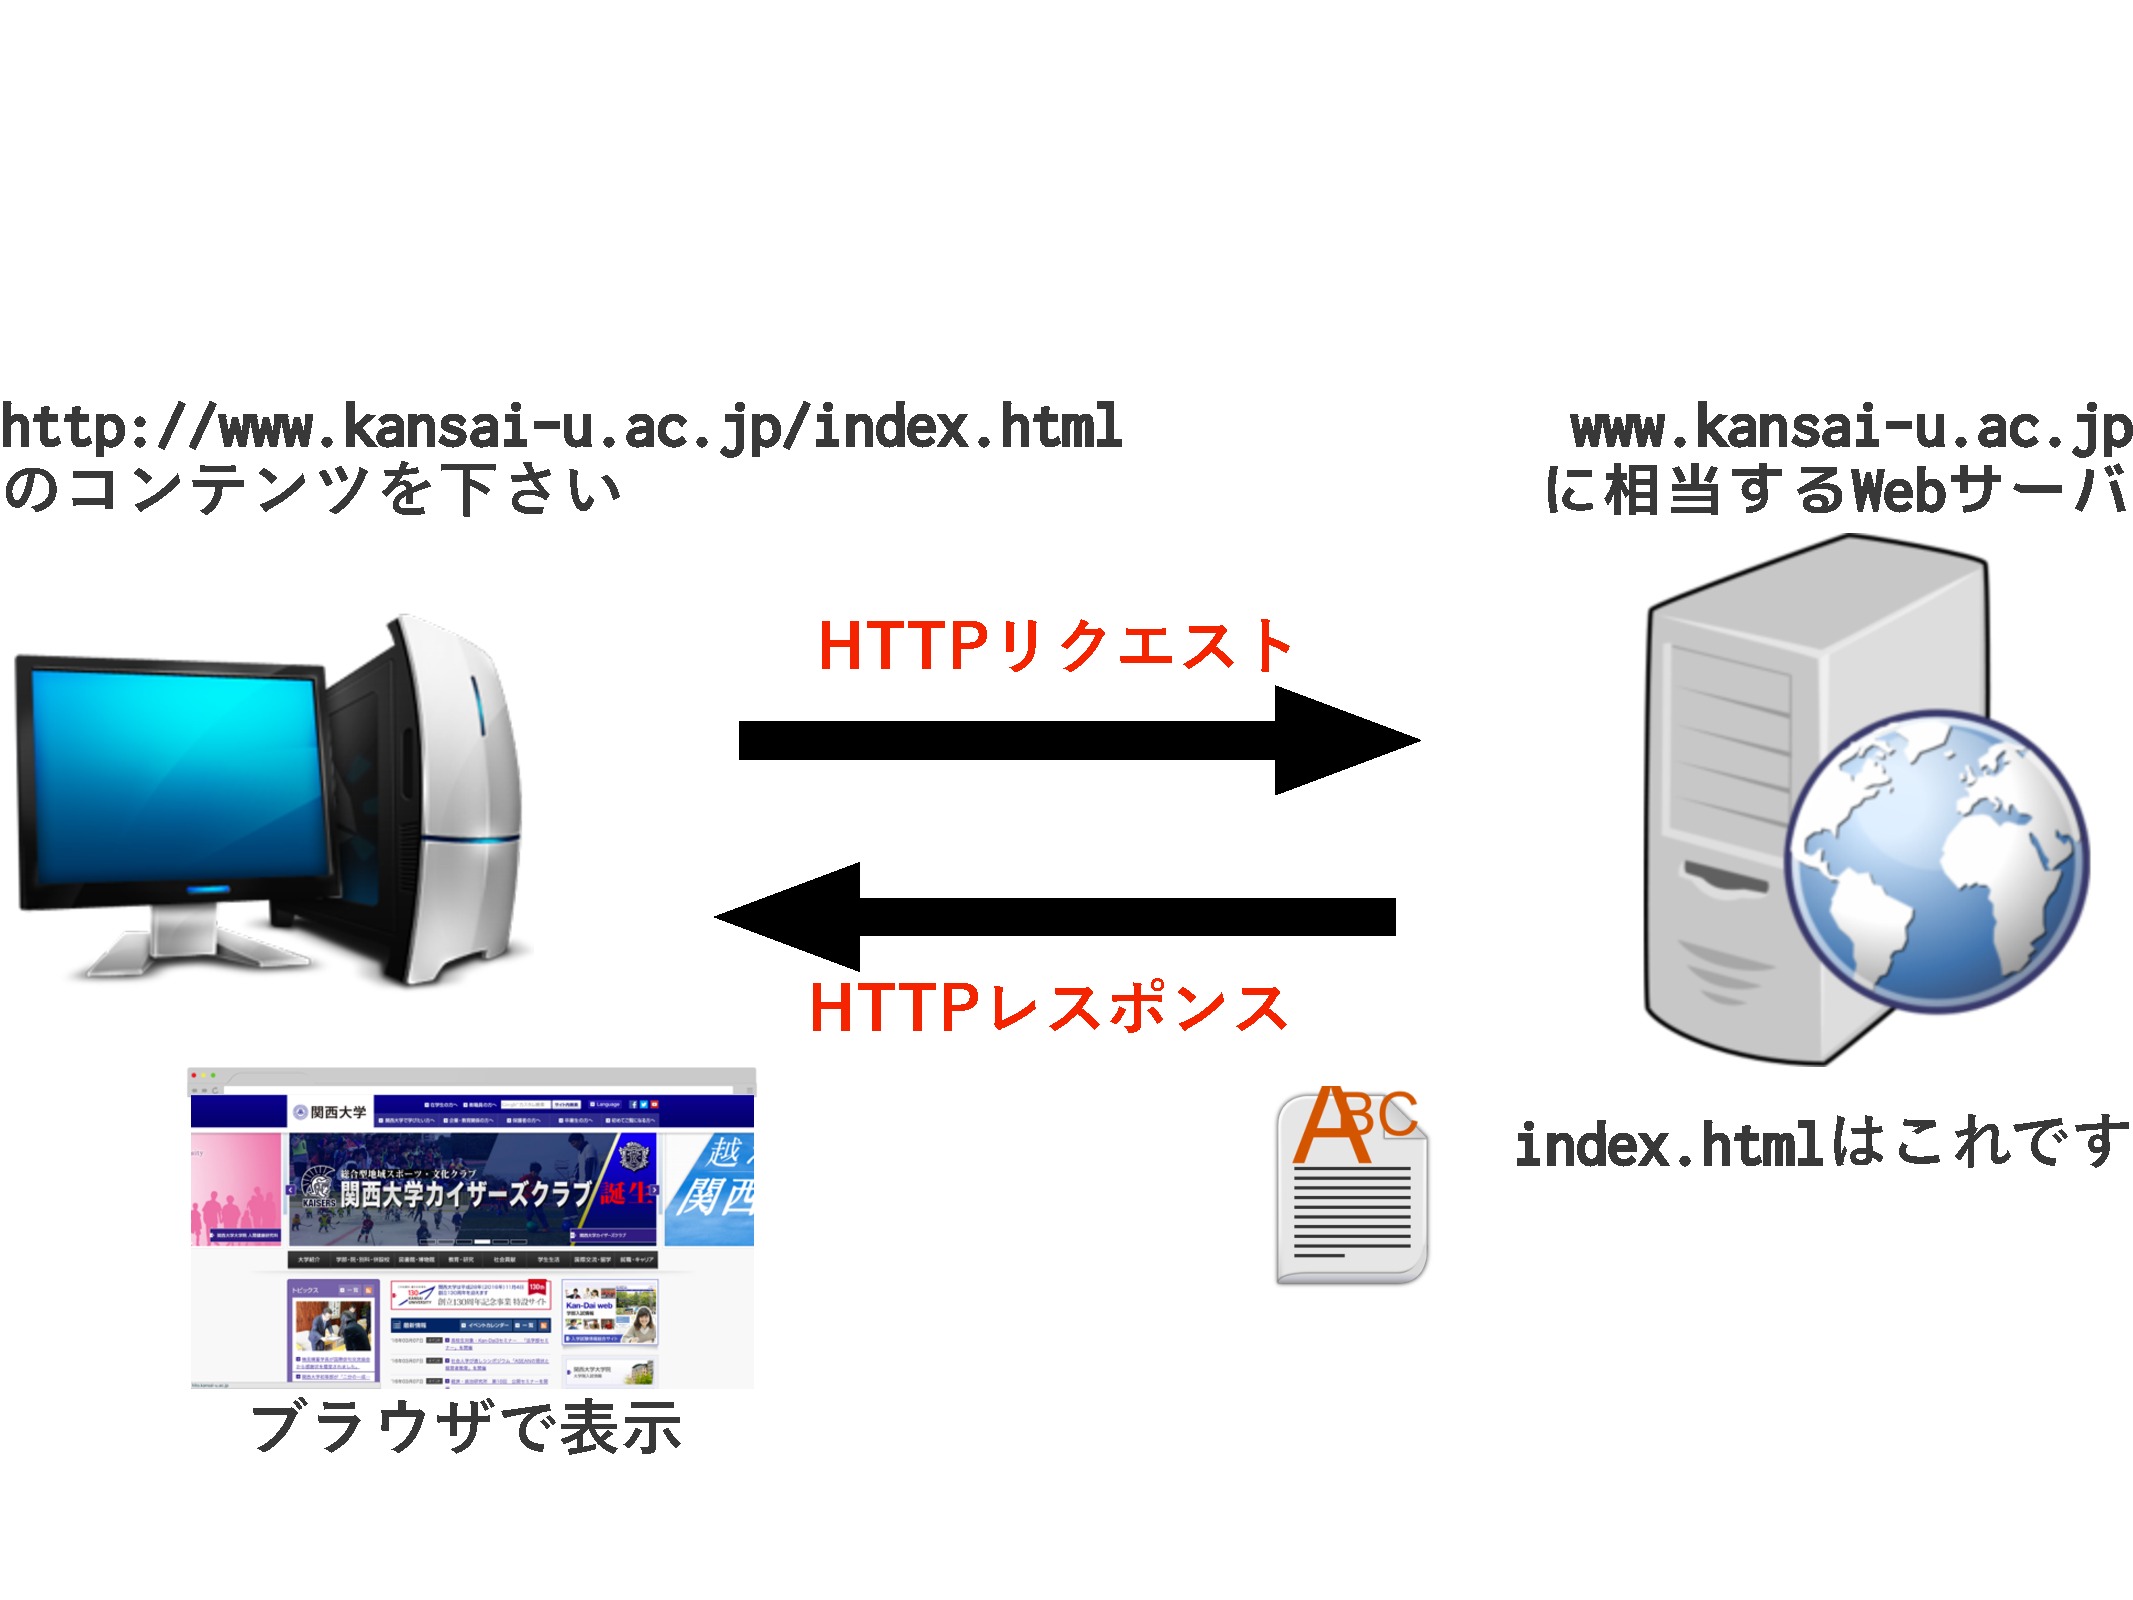
\includegraphics[width=0.9\hsize]{httpflow.pdf}
    \caption{HTTP通信の流れ}
    \label{fig:httpflow}
\end{figure}

また上記の例における通信をテキストベースで表現したものが,リスト\ref{list:httpreq}とリスト\ref{list:httpres}に当たる.
「/index.html」というURIに対して,「GET」というメソッドを用いて,
HTTP/1.1バージョンで通信をしているといった具合だ.HTTPメソッドについては,後述する.

\begin{lstlisting}[basicstyle=\ttfamily\small, numbers=none, frame=tlrb, caption=HTTPリクエスト, label=list:httpreq]
GET /index.html HTTP/1.1
Host: www.kansai-u.ac.jp
\end{lstlisting}

上述のリクエストに対するHTTPレスポンスが次のものになる.
\begin{lstlisting}[basicstyle=\ttfamily\small, numbers=none, frame=tlrb, caption=HTTPレスポンス, label=list:httpres]
HTTP/1.1 200 OK
Date: Wed, 09 Mar 2016 16:50:39 GMT
Server: Apache
Accept-Ranges: bytes
Content-Length: 30569
Connection: close
Content-Type: text/html
Content-Language: ja

<index.htmlのHTMLコード>
\end{lstlisting}

\subsubsection{HTTPヘッダ}
HTTPでは,リクエストとレスポンス双方の通信に,ヘッダと呼ばれるものを付けて通信を行う.
このヘッダを付けることによって,一つ一つの通信を詳細化することや区別すること,最適化することが可能となる.
表\ref{tab:reqheader}と表\ref{tab:resheader}に,主なHTTPヘッダとその用途を示す.
ここで挙げた以外にも様々なヘッダが用意されており,それらを用いることにより,効果的なHTTP通信を実現している.
例えば,HTTP通信を減らすためにブラウザにコンテンツをキャッシュしたいとき,
HTTPヘッダを使って,ある程度の操作が出来る.

\begin{table}[htbp]
    \centering
    \caption{HTTPリクエストヘッダ一覧}
    \label{tab:reqheader}
    \begin{tabular}{c|c} \hline
        ヘッダ & 用途 \\ \hline
        Host & リクエスト先のサーバ名を示す \\ \hline
        Cookie & クライアントの状態管理情報をサーバに送る \\ \hline
        Accept & クライアントの受け入れ可能コンテンツタイプを返す \\ \hline
        Authorization & クライアントの認証情報を返す \\ \hline
    \end{tabular}
\end{table}
\begin{table}[htbp]
    \centering
    \caption{HTTPレスポンスヘッダ一覧}
    \label{tab:resheader}
    \begin{tabular}{c|c} \hline
        ヘッダ & 用途 \\ \hline
        Server & Webサーバの情報を返す \\ \hline
        WWW-Authenticate & 認証領域名を示す固有値 \\ \hline
    \end{tabular}
\end{table}


\subsubsection{HTTPメソッド}
HTTPリクエストは,そのリクエストが何を意味しているかを示すために,メソッドと呼ばれる種類で分けられる.
主なメソッドとして,「GET」と「POST」が挙げられる.
通常,「GET」メソッドは,主にWebページ等のコンテンツを取得するときに使われ,
「POST」メソッドは,Webサーバにデータを送りたいときに使われる.
この他,「PUT」や「DELETE」,「HEAD」が存在する.
RESTful API等を考えない限り,現状変わった挙動はない.

\subsection{FTP}
FTPとは,File Transfer Protocolの略で,ネットワークを用いたファイル転送のためのプロトコルである.
主に,Web用のコンテンツファイル(HTMLファイルや画像等)をサーバ上にアップロードするときや,
フリーソフト等をクライアントがダウンロードしたいときなどに使われていた.
FTPは,プロトコル自体に暗号化の仕組みが存在しないため,HTTP同様に通信の盗聴が容易である.
セキュアな通信を確立するため,FTPに暗号化通信の仕組みを組み込んだFTPSや,後述するSSHという仕組みを用いて通信を暗号化するSFTPが存在する.

\subsection{SSH}
SSHとは,Secure Shellの略で,暗号化された通信上で,リモートコンピュータにログインするためのプロトコルである.
全ての通信は,ログインのためのパスワード情報等も含めて暗号化されているため,盗聴されていたとしても内容が漏洩する心配はない.
ログイン方法には,パスワードを使ったパスワード認証と公開鍵を用いた公開鍵認証があり,
認証情報をよりセキュアに管理するには公開鍵認証を使ったほうが良い.

SSHは,他のサービスとも一緒に使われることがあり,上述したFTPをSSH通信で実現するSFTPや,SFTPに似たものでリモートコンピュータ上に安全にファイルをコピーするためのscpというものが存在する.



%
%
% 編集者記録欄(学籍番号及び氏名).
\vspace{1cm}
\begin{table}[b]
  \begin{flushright}
    \begin{tabular}{llll}
      20XX年X月X日 & 初版 & XX-XXXX & 名無 権兵衛 \\
      20XX年Y月Y日 & 第二版 & YY-YYYY & John Smith
    \end{tabular}
  \end{flushright}
\end{table}

\end{document}
